% Options for packages loaded elsewhere
\PassOptionsToPackage{unicode}{hyperref}
\PassOptionsToPackage{hyphens}{url}
\PassOptionsToPackage{dvipsnames,svgnames,x11names}{xcolor}
%
\documentclass[
  letterpaper,
  DIV=11,
  numbers=noendperiod]{scrartcl}

\usepackage{amsmath,amssymb}
\usepackage{lmodern}
\usepackage{iftex}
\ifPDFTeX
  \usepackage[T1]{fontenc}
  \usepackage[utf8]{inputenc}
  \usepackage{textcomp} % provide euro and other symbols
\else % if luatex or xetex
  \usepackage{unicode-math}
  \defaultfontfeatures{Scale=MatchLowercase}
  \defaultfontfeatures[\rmfamily]{Ligatures=TeX,Scale=1}
\fi
% Use upquote if available, for straight quotes in verbatim environments
\IfFileExists{upquote.sty}{\usepackage{upquote}}{}
\IfFileExists{microtype.sty}{% use microtype if available
  \usepackage[]{microtype}
  \UseMicrotypeSet[protrusion]{basicmath} % disable protrusion for tt fonts
}{}
\makeatletter
\@ifundefined{KOMAClassName}{% if non-KOMA class
  \IfFileExists{parskip.sty}{%
    \usepackage{parskip}
  }{% else
    \setlength{\parindent}{0pt}
    \setlength{\parskip}{6pt plus 2pt minus 1pt}}
}{% if KOMA class
  \KOMAoptions{parskip=half}}
\makeatother
\usepackage{xcolor}
\setlength{\emergencystretch}{3em} % prevent overfull lines
\setcounter{secnumdepth}{-\maxdimen} % remove section numbering
% Make \paragraph and \subparagraph free-standing
\ifx\paragraph\undefined\else
  \let\oldparagraph\paragraph
  \renewcommand{\paragraph}[1]{\oldparagraph{#1}\mbox{}}
\fi
\ifx\subparagraph\undefined\else
  \let\oldsubparagraph\subparagraph
  \renewcommand{\subparagraph}[1]{\oldsubparagraph{#1}\mbox{}}
\fi


\providecommand{\tightlist}{%
  \setlength{\itemsep}{0pt}\setlength{\parskip}{0pt}}\usepackage{longtable,booktabs,array}
\usepackage{calc} % for calculating minipage widths
% Correct order of tables after \paragraph or \subparagraph
\usepackage{etoolbox}
\makeatletter
\patchcmd\longtable{\par}{\if@noskipsec\mbox{}\fi\par}{}{}
\makeatother
% Allow footnotes in longtable head/foot
\IfFileExists{footnotehyper.sty}{\usepackage{footnotehyper}}{\usepackage{footnote}}
\makesavenoteenv{longtable}
\usepackage{graphicx}
\makeatletter
\def\maxwidth{\ifdim\Gin@nat@width>\linewidth\linewidth\else\Gin@nat@width\fi}
\def\maxheight{\ifdim\Gin@nat@height>\textheight\textheight\else\Gin@nat@height\fi}
\makeatother
% Scale images if necessary, so that they will not overflow the page
% margins by default, and it is still possible to overwrite the defaults
% using explicit options in \includegraphics[width, height, ...]{}
\setkeys{Gin}{width=\maxwidth,height=\maxheight,keepaspectratio}
% Set default figure placement to htbp
\makeatletter
\def\fps@figure{htbp}
\makeatother

\usepackage{blkarray}
\KOMAoption{captions}{tableheading}
\makeatletter
\makeatother
\makeatletter
\makeatother
\makeatletter
\@ifpackageloaded{caption}{}{\usepackage{caption}}
\AtBeginDocument{%
\ifdefined\contentsname
  \renewcommand*\contentsname{Table of contents}
\else
  \newcommand\contentsname{Table of contents}
\fi
\ifdefined\listfigurename
  \renewcommand*\listfigurename{List of Figures}
\else
  \newcommand\listfigurename{List of Figures}
\fi
\ifdefined\listtablename
  \renewcommand*\listtablename{List of Tables}
\else
  \newcommand\listtablename{List of Tables}
\fi
\ifdefined\figurename
  \renewcommand*\figurename{Figure}
\else
  \newcommand\figurename{Figure}
\fi
\ifdefined\tablename
  \renewcommand*\tablename{Table}
\else
  \newcommand\tablename{Table}
\fi
}
\@ifpackageloaded{float}{}{\usepackage{float}}
\floatstyle{ruled}
\@ifundefined{c@chapter}{\newfloat{codelisting}{h}{lop}}{\newfloat{codelisting}{h}{lop}[chapter]}
\floatname{codelisting}{Listing}
\newcommand*\listoflistings{\listof{codelisting}{List of Listings}}
\makeatother
\makeatletter
\@ifpackageloaded{caption}{}{\usepackage{caption}}
\@ifpackageloaded{subcaption}{}{\usepackage{subcaption}}
\makeatother
\makeatletter
\@ifpackageloaded{tcolorbox}{}{\usepackage[many]{tcolorbox}}
\makeatother
\makeatletter
\@ifundefined{shadecolor}{\definecolor{shadecolor}{rgb}{.97, .97, .97}}
\makeatother
\makeatletter
\makeatother
\ifLuaTeX
  \usepackage{selnolig}  % disable illegal ligatures
\fi
\usepackage[]{natbib}
\bibliographystyle{plainnat}
\IfFileExists{bookmark.sty}{\usepackage{bookmark}}{\usepackage{hyperref}}
\IfFileExists{xurl.sty}{\usepackage{xurl}}{} % add URL line breaks if available
\urlstyle{same} % disable monospaced font for URLs
\hypersetup{
  colorlinks=true,
  linkcolor={blue},
  filecolor={Maroon},
  citecolor={Blue},
  urlcolor={Blue},
  pdfcreator={LaTeX via pandoc}}

\author{}
\date{}

\begin{document}
\ifdefined\Shaded\renewenvironment{Shaded}{\begin{tcolorbox}[boxrule=0pt, enhanced, borderline west={3pt}{0pt}{shadecolor}, interior hidden, breakable, sharp corners, frame hidden]}{\end{tcolorbox}}\fi

\hypertarget{title-reintroduction-of-resistant-frogs-facilitates-landscape-scale-recovery-in-the-presence-of-a-lethal-fungal-disease}{%
\subsection{Title: Reintroduction of resistant frogs facilitates
landscape-scale recovery in the presence of a lethal fungal
disease}\label{title-reintroduction-of-resistant-frogs-facilitates-landscape-scale-recovery-in-the-presence-of-a-lethal-fungal-disease}}

\hypertarget{authors}{%
\subsubsection{Authors:}\label{authors}}

Roland A. Knapp\textsuperscript{a,b,}*, Mark Q.
Wilber\textsuperscript{c,1}, Allison Q. Byrne\textsuperscript{d,e,1},
Maxwell B. Joseph\textsuperscript{f,g}, Thomas C.
Smith\textsuperscript{a,b}, Andrew P. Rothstein\textsuperscript{d,e,h},
Robert L. Grasso\textsuperscript{i}, Erica Bree
Rosenblum\textsuperscript{d,e}

\hypertarget{affiliations}{%
\subsubsection{Affiliations:}\label{affiliations}}

\textsuperscript{a}Sierra Nevada Aquatic Research Laboratory, University
of California, Mammoth Lakes, CA, 93546

\textsuperscript{b}Earth Research Institute, University of California,
Santa Barbara, CA, 93106-3060

\textsuperscript{c}School of Natural Resources, University of Tennessee
Institute of Agriculture, Knoxville, TN, 37996

\textsuperscript{d}Department of Environmental Science, Policy, and
Management, University of California - Berkeley, Berkeley, CA,
94720-3114

\textsuperscript{e}Museum of Vertebrate Zoology, University of
California - Berkeley, Berkeley, CA, 94720-3160

\textsuperscript{f}Earth Lab, University of Colorado, Boulder, CO, 80303

\textsuperscript{g}Current affiliation: Planet, San Francisco, CA, 94107

\textsuperscript{h}Current affiliation: Ginkgo Bioworks, Boston, MA,
02210

\textsuperscript{i}Resources Management and Science, Yosemite National
Park, El Portal, CA, 95318

*Corresponding author: Sierra Nevada Aquatic Research Laboratory, 1016
Mount Morrison Road, Mammoth Lakes, CA 93546, phone: 760.647.0034,
email: roland.knapp@ucsb.edu

\textsuperscript{1}These authors contributed equally to this work.

\textbf{Classification:} Biological Sciences - Ecology

\textbf{Key words:} evolution, resistance, amphibians, population
recovery, reintroduction, disease, \emph{Batrachochytrium dendrobatidis}

\hypertarget{abstract}{%
\subsubsection{Abstract}\label{abstract}}

Vast alteration of the biosphere by humans is causing a sixth mass
extinction, driven in part by an increase in emerging infectious
diseases. The emergence of the lethal fungal pathogen
(\emph{Batrachochytrium dendrobatidis}; ``Bd'') has devastated global
amphibian biodiversity, with hundreds of species experiencing declines
or extinctions. With no broadly applicable methods available to reverse
these impacts in the wild, the future of many amphibians appears grim.
The once-common mountain yellow-legged (MYL) frog is emblematic of
amphibians threatened by Bd. Although most MYL frog populations are
extirpated following disease outbreaks, some persist and eventually
recover. Frogs in these recovering populations have increased resistance
against Bd infection, consistent with evolution of resistant genotypes
and/or acquired immunity. We conducted a 15-year landscape-scale
reintroduction study and show that frogs collected from recovering
populations and reintroduced to vacant habitats can reestablish
populations despite the presence of Bd. In addition, results from
viability modeling suggest that many reintroduced populations have a low
probability of extinction over 50 years. To better understand the role
of evolution in frog resistance, we compared the genomes of MYL frogs
from Bd-naive and recovering populations. We found substantial
differences between these categories, including changes in immune
function loci that may confer increased resistance, consistent with
evolutionary changes in response to Bd exposure. These results provide a
rare example of how reintroduction of resistant individuals can allow
the landscape-scale recovery of disease-impacted species. This example
has broad implications for the many taxa worldwide that are threatened
with extinction by novel pathogens.

\hypertarget{significance}{%
\subsubsection{Significance}\label{significance}}

Understanding how species persist despite accelerating global change is
critical for the conservation of biodiversity. Emerging infectious
diseases can have particularly devastating impacts, and few options
exist to reverse these effects. We used large-scale reintroductions of
disease-resistant individuals in an effort to recover a once-common frog
species driven to near-extinction by a disease that has decimated
amphibian biodiversity. Introduction of resistant frogs allowed
reestablishment of viable populations in the presence of disease. In
addition, resistance may be at least partially the result of natural
selection at specific immune function genes, which show evidence for
selection in recovering populations. The evolution of resistance and
reintroduction of resistant individuals could play an important role in
biodiversity conservation in our rapidly changing world.

\hypertarget{introduction}{%
\subsubsection{Introduction}\label{introduction}}

Human activities are increasingly impacting global biodiversity
\citep{ceballos2015}, with important implications for ecosystem
resilience and human welfare \citep{naeem2009}. One consequence of human
alteration of the biosphere is an increase in emerging infectious
diseases \citep{jones2008, fisher2012}. Such diseases pose a severe
threat to wildlife populations \citep{daszak2000}, and have caused
dramatic declines and extinctions in a wide range of taxa, including
echinoderms, mammals, birds, and amphibians
\citep{hewson2014, samuel2015, scheele2019, cunningham2021}. Amphibians
are experiencing particularly devastating impacts of disease due to the
recent emergence and global spread of the highly virulent amphibian
chytrid fungus, \emph{Batrachochytrium dendrobatidis} (Bd)
\citep{luedtke2023, scheele2019}. By one estimate, hundreds of species
have experienced Bd-caused declines, and numerous susceptible taxa are
extinct in the wild \citep{scheele2019}. These impacts to global
biodiversity may be unprecedented, and highlight the importance of
understanding mechanisms of species persistence in the presence of
emerging diseases \citep{russell2020}.

Evidence of natural recovery in the many Bd-impacted amphibian
populations is surprisingly rare \citep[for notable exceptions,
see][]{scheele2017, voyles2018, knapp2016}, suggesting that
disease-caused declines will be difficult to reverse. This apparent low
resilience to disease effects may be due to the limited ability of many
amphibians to develop Bd resistance and/or tolerance, which in turn,
could also lessen the effectiveness of potential Bd mitigation
strategies. Following pathogen arrival in a host population, resistance
(ability to limit pathogen burden) and tolerance (ability to limit the
harm caused by a particular burden) are key mechanisms to reduce disease
impacts \citep{raberg2009} and facilitate population persistence and
recovery \citep{brannelly2021}. Host immunity and evolution both play
important roles in the development of resistance and tolerance, and
utilizing these factors would seem a promising approach to developing
effective strategies to mitigate disease impacts in the wild
\citep{garner2016, woodhams2011}. However, several aspects of the
amphibian-Bd system present difficult obstacles, including (i) the
general inability of amphibians to mount an effective immune response
against Bd infection \citep{rosenblum2012, fites2013, grogan2018a}, and
(ii) the apparent rarity of evolution of more resistant/tolerant
genotypes \citep[but see][]{savage2016, grogan2018b}. These factors
suggest that reintroduction of amphibians into sites to reestablish
populations extirpated by Bd will often result not in population
recovery, but instead in the rapid reinfection and mortality of the
introduced animals and/or their progeny
\citep{hammond2021, knapp2022, stockwell2008, scheele2021}. If true, the
future of many amphibian species threatened by Bd appears bleak.

The mountain yellow-legged (MYL) frog, composed of the sister species
\emph{Rana muscosa} and \emph{Rana sierrae} \citep{vredenburg2007}, is
emblematic of the global declines of amphibians caused by Bd
\citep{scheele2019}. Once the most common amphibian in the high
elevation portion of California's Sierra Nevada mountains
\citep[USA,][]{grinnell1924}, during the past century this frog has
disappeared from more than 90\% of its historical range
\citep{vredenburg2007}. Due to the severity of its decline and the
increasing probability of extinction, both species are now listed as
``endangered'' under the U.S. Endangered Species Act. In the Sierra
Nevada, this decline was initiated by the introduction of non-native
trout into the extensive historically-fishless region
\citep{bradford1989, knapp2000} starting in the late 1800s. The arrival
of Bd in the mid-1900s and its subsequent spread \citep{vredenburg2019}
caused additional large-scale population extirpations
\citep{vredenburg2010, rachowicz2006}. These Bd-caused declines are
fundamentally different from the fish-caused declines because fish
eradication is feasible \citep{knapp1998} and results in the rapid
recovery of frog populations \citep{knapp2007, vredenburg2004}. In
contrast, Bd appears to persist in habitats even in the absence of
amphibian hosts \citep{walker2007}, and therefore represents a long-term
alteration of invaded ecosystems that amphibians will need to overcome
to reestablish populations.

Despite the catastrophic impact of Bd on MYL frogs, wherein most
Bd-naive populations are extirpated following Bd arrival
\citep{vredenburg2010}, some populations have persisted after epizootics
\citep[during which Bd infection intensity on frogs is very
high,][]{briggs2010} and are now recovering
(Figure~\ref{fig-recovery-model}) \citep{knapp2016}. Frogs in these
recovering populations show reduced susceptibility to Bd infection
\citep{knapp2016}, with infection intensity (``load'') on adults
consistently in the low-to-moderate range
\citep{briggs2010, knapp2011, joseph2018}. This reduced susceptibility
is evident even under controlled laboratory conditions
\citep{knapp2016}, indicative of host resistance against Bd infection
(and not simply an effect of factors external to individual frogs, e.g.,
environmental conditions). In addition to frogs from recovering
populations having higher resistance to Bd infection than those from
naive populations, they could also have higher tolerance, but no data
are currently available to evaluate this possibility. Therefore, we
focus on resistance throughout this paper. The observed resistance of
MYL frogs could be the result of several non-mutually exclusive
mechanisms, including natural selection for more resistant genotypes
\citep{savage2016, grogan2018b}, acquired immunity \citep{grogan2018a},
and/or inherent between-population differences that pre-date Bd
exposure. The possible evolution of MYL frog resistance and subsequent
population recovery is consistent with that expected under
``evolutionary rescue'', whereby rapid evolutionary change increases the
frequency of adaptive alleles and restores positive population growth
\citep{carlson2014, searle2020}. This intriguing possibility also
suggests an opportunity to expand recovery beyond the spatial scale
possible under natural recovery by utilizing resistant frogs from
recovering populations in reintroductions to vacant habitats
(Figure~\ref{fig-recovery-model}) \citep{joseph2018, mendelson2019}.

In the current study, we had three primary objectives. First, to
determine whether the reintroduction of resistant MYL frogs obtained
from populations recovering from Bd-caused declines allows the
successful reestablishment of extirpated populations despite ongoing
disease, we conducted a 15-year landscape-scale frog reintroduction
effort (Figure~\ref{fig-recovery-model}). Second, to extend our
inferences of population recovery well beyond the temporal extent of our
reintroduction study, we developed a model to estimate the probability
of persistence for the reintroduced populations over a multi-decadal
period (Figure~\ref{fig-recovery-model}). Third, given the importance of
resistance for frog survival, population establishment, and long-term
viability (this study), we conducted a genomic study using exome capture
methods to determine whether MYL frogs in recovering populations show
evidence of selection and whether these genomic changes are associated
with resistance (Figure~\ref{fig-recovery-model}).

\hypertarget{results}{%
\subsubsection{Results}\label{results}}

\hypertarget{frog-population-recovery}{%
\paragraph{Frog population recovery}\label{frog-population-recovery}}

To determine whether MYL frogs from recovering populations can be used
to reestablish extirpated populations, we conducted 24 reintroductions
in Yosemite National Park (2006--2020). Each of the reintroductions
involved collection of adult frogs from 1 of 3 recovering, Bd-positive
``donor'' populations and translocating them to 1 of 12 nearby recipient
sites (Figure~\ref{fig-yosemap} SI). The donor populations included 2 of
the 5 recovering populations used in the frog evolution study referenced
above (Figure~\ref{fig-allelefrequencies}: population 1 and 4), and
these donor populations contributed frogs for 20 of the 24
translocations. Following translocation, we estimated adult survival and
recruitment of new adults from capture-mark-recapture (CMR) surveys and
obtained counts of tadpoles and juveniles from visual encounter surveys
(VES). Across all translocation sites, the duration of survey time
series was 1--16 years (median = 5).

Of the 12 reintroduced populations, 9 (0.75) showed evidence of
successful reproduction in subsequent years, as indicated by the
presence of tadpoles and/or juveniles. For these 9 populations, one or
both life stages were detected in nearly all survey-years following
translocation (proportion of survey-years: median = 0.9, range =
0.29--1). These same populations were also those in which recruitment of
new adults (i.e., progeny of translocated individuals) was detected. As
with early life stages, recruits were detected in the majority of
post-translocation survey-years (proportion of survey-years: median =
0.79, range = 0.12--1). In summary, survey results indicate that
translocations resulted in the establishment of reproducing MYL frog
populations at most recipient sites despite the ongoing presence of Bd.

Bd loads were fairly consistent before versus after translocation, and
loads were nearly always well below the level indicative of severe
chytridiomycosis (i.e., the disease caused by Bd) and associated frog
mortality (Figure~\ref{fig-bdload-beforeafter} SI)
\citep{joseph2018, vredenburg2010}. Although it is possible that the
observed relatively small changes in load are a consequence of
individuals with high Bd loads dying and therefore being unavailable for
sampling during the post-translocation period, the fact that there was
little difference in pre- versus post-translocation Bd loads even in
those populations that had very high frog survival (70556, 74976 - see
below; Figure~\ref{fig-bdload-beforeafter} SI) suggests a true lack of
substantial change in Bd load.

The ultimate measure of reintroduction success is the establishment of a
self-sustaining population. Given that it can take years or even decades
to determine the self-sustainability of a reintroduced population
\citep[for an example in MYL frogs, see][]{joseph2018}, the use of
proxies is essential for providing shorter-term insights into
reintroduction success and the factors driving it. Results from our CMR
surveys allowed us to accurately estimate frog survival, including over
the entire CMR time series for each site and during only the 1-year
period immediately following translocation. These estimates were made
using site-specific models analyzed using the mrmr package. We use these
estimates to describe general patterns of frog survival in all
translocated cohorts, and in an among-site meta-analysis of frog
survival to identify important predictors of 1-year frog survival (e.g.,
Bd load).

Estimates of 1-year frog survival indicate that survival was highly
variable between recipient sites, but relatively constant within
recipient sites (for the subset of sites that received multiple
translocations; Figure~\ref{fig-translocation-survival}). These patterns
indicate an important effect of site characteristics on frog survival.
In addition, 1-year survival was higher for frogs translocated later in
the study period than earlier: 5 of the 7 populations translocated after
2013 had estimated survival \(\ge\) 0.5, compared to only 1 of 5
populations translocated prior to 2013. We suggest this resulted
primarily from our improved ability to choose recipient sites with
higher habitat quality for \emph{R. sierrae} (see \textbf{Materials and
Methods - Frog population recovery - Field methods} for details). This
increased survival has direct implications for population viability (see
\textbf{Results - Long-term population viability}).

The goal of our meta-analysis was to identify important predictors of
1-year frog survival. We were particularly interested in whether Bd load
had a negative effect on adult survival, as would be expected if frogs
were highly susceptible to Bd infection. This analysis was conducted in
a Bayesian framework and included a diversity of site, cohort, and
individual-level characteristics as predictors and 1-year frog survival
(Figure~\ref{fig-translocation-survival}) as the response variable. The
best model of 1-year frog survival identified several important
predictors, but Bd load at the time of translocation was not among them
(Figure~\ref{fig-survival-postdens} SI). Instead, important predictors
included winter severity in the year following translocation (snow\_t1),
site elevation, and donor population (Figure~\ref{fig-cond-effects},
Figure~\ref{fig-survival-postdens} SI). Males had somewhat higher
survival than females, but this effect was small
(Figure~\ref{fig-cond-effects}, Figure~\ref{fig-survival-postdens} SI).
The absence of Bd load as an important predictor of frog survival is
consistent with frogs in recovering populations having sufficient
resistance to suppress Bd loads below harmful levels.

In summary, results from our frog translocation study indicate that
translocations resulted in (i) relatively high 1-year survival of
translocated adults, as well as reproduction and recruitment, at the
majority of recipient sites, (ii) 1-year survival of adults is
influenced by site characteristics, weather conditions, and donor
population (but not Bd load), and (iii) based on the relatively small
changes in Bd load after translocation, loads appear more strongly
influenced by frog characteristics (e.g., resistance) than site
characteristics. Together, these results indicate that frogs
translocated from recovering populations can maintain the benefits of
resistance in non-natal habitats. In addition, in 3 locations where
longer CMR time series allowed us to assess the survival of new adults
recruited to the population, naturally-recruited adults had equivalent
or higher survival probabilities than the originally translocated adults
(Figure~\ref{fig-compare_surv_probs} SI). This suggests that frog
resistance is maintained across generations. All of the conditions
described above are supportive of population establishment and long-term
population growth.

\hypertarget{long-term-population-viability}{%
\paragraph{Long-term population
viability}\label{long-term-population-viability}}

Results from the frog translocation study indicated that most
populations showed evidence of successful reproduction and recruitment,
and that adult survival was often relatively high (described above).
Although suggestive of population establishment, a decade or more of
surveys may be necessary to confirm that populations are in fact
self-sustaining \citep{joseph2018}. To extend our inferences of
population establishment beyond those possible from the site-specific
CMR data, we developed a population viability model. Specifically, to
test whether the observed yearly adult survival probabilities in
translocated populations were sufficient for long-term viability, we
built a stage-structured matrix model that captured known frog
demography and included demographic and environmental stochasticity. We
parameterized the model using CMR data from translocated populations and
known life history values in this system (Table~\ref{tbl-param_values}
SI).

Given observed yearly adult survival probabilities of translocated frogs
(from site-specific mrmr CMR models; provided in legend of
Figure~\ref{fig-viability} B) and a yearly survival probability of the
year-1 juvenile class (\(\sigma_{J_1}\)) greater than 0.09, at least six
of twelve translocated populations should experience a long-run growth
rate \(\lambda\) greater than 1 in the presence of Bd
(Figure~\ref{fig-viability} A; median predicted \(\lambda\) ranges from
1.19-1.40 for these six populations). These six populations all had
observed yearly adult survival greater than 0.5. As year-1 juvenile
survival probability increased above 0.2, the deterministic long-run
growth rate of eight of twelve population was greater than 1
(Figure~\ref{fig-viability} A).

Even when incorporating (i) demographic stochasticity and (ii)
environmental stochasticity in year-1 juvenile survival and recruitment
(the transition that we expect to be the most subject to environmental
variability in the presence of Bd), populations with high adult survival
are likely to persist over a 50 year time horizon. Our model predicted
that, following a single introduction of 40 adult individuals into a
population, the six populations with the highest adult survival
probabilities (\(\sigma_{A_R} > 0.5\)) had 50-year extinction
probabilities of less than 0.5 when the average year-1 juvenile survival
was greater than 0.10 (Figure~\ref{fig-viability} B). This indicates
strong potential for long-term persistence in the presence of Bd and
environmental variability in survival and recruitment. In contrast, for
the six populations where yearly adult survival probability
\(\sigma_{A_R} < 0.5\), extinction probability over 50 years was always
predicted to be \textgreater{} 50\% regardless of the value of mean
year-1 juvenile survival between 0 and 0.25. To test the validity of our
model predictions, we demonstrated that our stochastic model could
describe the general recovery trajectory of our translocated population
with the longest survey history (Figure~\ref{fig-viability} C;
population 70550, surveyed for 16 years).

In summary, our model demonstrates that given observed yearly adult
survival probabilities of translocated frogs, 50\% of our translocated
populations have a high probability of population growth and long-term
viability in the presence of Bd. This is likely a conservative estimate
because there is evidence that naturally-recruited adults have higher
survival probability than translocated adults
(Figure~\ref{fig-compare_surv_probs} SI), but we considered these
probabilities to be equal in all but three of our populations where we
had sufficient data to distinguish these different probabilities.

\hypertarget{frog-evolution-in-response-to-bd}{%
\paragraph{Frog evolution in response to
Bd}\label{frog-evolution-in-response-to-bd}}

Results from the preceding sections indicate the critical role of frog
resistance in post-translocation frog survival, population growth, and
population viability. As such, identifying the mechanisms underlying
this resistance would fill a key gap in our understanding of the factors
that promote population resilience in the presence of disease. Although
natural selection for more resistant frog genotypes, and evolutionary
rescue, may be foundational to the ability of frogs to recover despite
ongoing Bd infection, for MYL frogs the role of disease-mediated
selection in these processes remains unknown.

To determine whether MYL frog populations show genomic patterns
consistent with an evolutionary response to Bd, we compared frog exomes
(i.e., coding region of a genome) between populations with contrasting
histories of Bd exposure. Specifically, we compared frog genomes sampled
in 4 populations that have not yet experienced a Bd-caused epizootic
(``naive'') \citep{zhou2015} versus in 5 populations that experienced a
Bd epizootic during the past several decades and have since recovered to
varying degrees (``recovering''; Figure~\ref{fig-allelefrequencies})
\citep{knapp2016, vredenburg2010}. Bd-exposure histories of the 9 study
populations are based on 10-20 years of VES and Bd surveillance using
skin swabbing \citep[e.g.,][]{knapp2016, zhou2015, wilber2022}. Naive
populations are characterized by large numbers of adults (i.e, typically
1000s), Bd prevalence that is generally 0\% except during occasional Bd
failed invasions \citep[during which Bd loads remain very
low,][]{wilber2022}, and no history of Bd epizootics since we first
surveyed these populations in the late 1990s and early 2000s
\citep{zhou2015}. In contrast, recovering populations exist in an
enzootic state \citep{briggs2010}, characterized by smaller numbers of
adults (generally \textless{} 500), high Bd prevalence \citep[often
\textgreater{} 80\%,][]{knapp2011}, and, in adults, moderate Bd loads
that are typically well below the level expected to cause mortality
\citep{vredenburg2010}. Naive and recovering populations can be
identified unambiguously using these differences in Bd prevalence and
load. Finally, there is no potential for frog dispersal between the 9
study populations due to intervening distances and topography, as well
as the presence of introduced (predatory) fish and fish-induced habitat
fragmentation. (See \textbf{Supporting Information - Frog evolution in
response to Bd - Study design} for additional details regarding the
study design.)

We conducted a principal component analysis (PCA) of the genomic data to
describe the relationships between sampled populations, and then used
two complementary approaches to identify regions of the genome that
differed between naive and recovering populations (i.e., regions under
selection). First, we used a multivariate linear mixed model to evaluate
associations between population type (i.e., naive versus recovering) and
individual variants, including single nucleotide polymorphisms (SNPs)
and insertions/deletions (INDELS), while accounting for population
structure. Second, we used a splined window analysis to identify larger
genomic regions showing differences between population types in
\emph{F\textsubscript{ST}} and nucleotide diversity (\(\pi_{diff}\) =
\(\pi_{naive}\) - \(\pi_{recovering}\)).

Individual frogs clustered into 3 separate groups in principal component
space (Figure~\ref{fig-selectionresults} A SI), and clusters reflected
the species split (i.e., \emph{R. muscosa} versus \emph{R. sierrae}) and
the strong signature of isolation-by-distance that is characteristic of
MYL frogs \citep{rothstein2020, poorten2017, byrne2023}. Importantly,
each cluster contained at least one population from both the naive and
recovering groups, allowing us to distinguish allelic associations of
individuals sampled in the 2 population types versus allelic
associations resulting from population structure and genetic drift.

Results from the individual variant and splined window analyses show
that recovering populations have signatures of selection on multiple
regions of the genome. The analysis of individual variants identified 11
``outlier'' SNPs (i.e., showing significantly different allele
frequencies between naive versus recovering populations) from 7 distinct
genes across 4 contigs (Figure~\ref{fig-selectionresults} B, C SI). One
of the 7 identified genes (LOC108802036) does not have an associated
annotation. For the outlier SNPs, frequency differences between the
naive and recovering populations ranged from 0.41 to 0.86. Most of these
SNPs showed frequency differences in only a subset of the sampled
populations (Figure~\ref{fig-allelefrequencies} A, B), but the SNP in
the RIN3 gene showed consistent differences in frequencies across all
populations (Figure~\ref{fig-allelefrequencies} C). This is suggestive
of parallel selection at this locus across multiple populations. The
other 6 outlier variants showed less consistent frequency differences
across the study populations, but for these we still found a
statistically significant signal of selection in 2 of the 3 genetic
clusters (containing populations 5--9;
Figure~\ref{fig-allelefrequencies}, Figure~\ref{fig-selectionresults} A
SI). Therefore, although some outlier variant associations have a more
limited geographic extent than RIN3, they still describe results that
suggest parallel evolutionary changes following Bd exposure.

The splined window analysis identified 33 outlier regions for
\(\pi_{diff}\) and 58 outlier regions for \emph{F\textsubscript{ST}}
(Figure~\ref{fig-spline-manhattan} A, B). Of these, 9 regions were
outliers for both metrics (``shared regions'') and 2 of these shared
regions also contained one or more of the outlier SNPs described above.
A total of 35 annotated genes were found in the 9 shared regions. Given
this large number of genes, here we focus on those with the strongest
signal of selection and/or immune-related functions. The largest
\(\pi_{diff}\), indicative of directional selection, occurred in a 163kb
region on Contig19, 12.9Mb upstream of the RIN3 outlier SNP
(Figure~\ref{fig-spline-manhattan} C). This region contains
approximately 500 SNPs and one annotated gene called
``interferon-induced very large GTPase 1-like'' (GVINP1). Additionally,
a shared outlier region on Contig1 contained two complement factor genes
(C6 and C7). Interestingly, this region had a large negative
\(\pi_{diff}\) value, consistent with balancing selection. Finally, one
shared outlier region on Contig8 contained one outlier SNP (TCF19) and
was within 360kb of another outlier SNP (VARS)
(Figure~\ref{fig-spline-manhattan} D, Figure~\ref{fig-synteny-plot} SI).
This region (854kb from the beginning of the outlier window to the VARS
SNP) contained a total of 8 annotated genes. In \emph{Xenopus}, five of
these genes occur in the extended major histocompatibility complex (MHC)
Class I region (FLOT1, TUBB, MDC1, CCHCR1, TCF19) and three occur in the
extended MHC Class III region (HSP70, LSM2, VARS) \citep{ohta2006}.
Therefore, this region under selection is part of the extended MHC Class
I and III complex and shows synteny with other amphibian genomes.

Although the joint processes of Bd-caused population declines and
selection in response to Bd exposure could affect genetic diversity of
recovering populations, we found no consistent differences in
individual-level heterozygosity or population-level \(\pi\) between
naive and recovering populations (see \textbf{Supporting Information -
Frog evolution in response to Bd - Genetic diversity} for details).
Thus, despite localized selection in particular regions of the genome,
we did not find evidence for reduced genetic diversity across the genome
in recovering populations. In addition, no gene ontology (GO) biological
functions, molecular functions, or cellular processes were
over-represented in either the outlier variants or the 35 genes located
in the overlapping \emph{F\textsubscript{ST}} and \(\pi_{diff}\) splined
windows (see \textbf{Supporting Information - Frog evolution in response
to Bd} \textbf{- GO analysis} for details).

In summary, our genomic results indicate that the exomes of frogs from
naive and recovering populations show substantial differences,
consistent with parallel evolutionary changes following Bd exposure. The
regions under selection contain several immunologically-relevant genes
and gene families that are directly linked to disease resistance in
other taxa.

\hypertarget{discussion}{%
\subsubsection{Discussion}\label{discussion}}

Disease-induced population declines are decimating global biodiversity
\citep{daszak2000}, but broadly-applicable strategies to recover
affected species are generally lacking \citep[e.g.,][]{garner2016}.
Here, we tested the possibility that populations of resistant
individuals from naturally recovering populations can be used to
reestablish extirpated populations of the endangered MYL frog in the
presence of a highly virulent fungal pathogen (Bd). Our results indicate
(i) the capacity of reintroduced populations to become established and
eventually recover despite ongoing disease, (ii) that the recovering
populations are likely to persist over a 50-year period, (iii) that
there are substantial genomic differences between naive and recovering
MYL frog populations, consistent with evolutionary change in frogs
following Bd exposure, and (iv) that some of the genomic regions under
selection contain genes related to disease resistance. Collectively,
these results (Figure~\ref{fig-recovery-model}) provide a rare example
of amphibian recovery in the presence of Bd, and have important
implications for the conservation and recovery of amphibians and other
taxa worldwide that are endangered by escalating impacts from emerging
infectious diseases. In light of the generally low success rate of
amphibian reintroduction efforts \citep{dodd2005}, our success in
reestablishing MYL frog populations via translocation of resistant
individuals is striking, and even more so given that MYL frogs were
driven to near-extinction by Bd.

In the following discussion, we follow the sequence of frog recovery
described in Figure~\ref{fig-recovery-model} to structure our key
points. Previous field studies in MYL frogs show that frog-Bd dynamics
and frog survival in the presence of Bd are fundamentally different
between naive and recovering populations. Following the arrival and
establishment of Bd in previously-naive populations, adult frogs develop
high Bd loads that lead to mass die-offs \citep{vredenburg2010}. In
contrast, in recovering populations adult frogs typically have
low-to-moderate and relatively constant Bd loads and mass die-offs are
not observed \citep[see also Figure~\ref{fig-bdload-beforeafter}
SI]{briggs2010, knapp2011}. The differences in Bd load of frogs from
naive and recovering populations are also observed in controlled
laboratory studies \citep[see Figure 4 in][]{knapp2016}, and clearly
indicate that frogs from recovering populations exhibit resistance
against Bd infection. This resistance could in theory be due to several
factors, including natural selection for more resistant genotypes,
acquired immunity, and/or inherent between-population differences that
pre-date Bd exposure, but until now evidence to evaluate the role of
evolution was lacking.

Results from our genomic analyses suggest that natural selection for
adaptive alleles is at least partially responsible for the increased
resistance of frogs in recovering populations. We identified multiple
specific alleles and genomic regions showing signatures of selection
between adjacent naive and recovering MYL frog populations, consistent
with selection following Bd exposure. These analysis are based on
samples collected from virtually all of the MYL frog populations
remaining in a naive state, as well as adjacent recovering populations.
This study design produced genetic clusters that each contained at least
one naive and one recovering population, allowing us to detect selection
without the confounding effects of population structure. In addition, we
did not find a reduction in overall genetic variation in the recovering
populations, suggesting that despite localized selection in the genome,
these populations retain adequate genetic diversity for long-term
persistence.

Importantly, some genomic regions that we identified as under selection
are associated with cellular and immunological mechanisms known to
contribute to disease resistance, including in amphibians
\citep{zamudio2020}. For example, the MHC plays an important role in
immunity. In our study, we identified a region that shows evidence of
selection in recovering populations and contains eight genes associated
with either the MHC Class I or Class III regions. These results
corroborate numerous previous studies linking MHC genes to amphibian
resistance against Bd \citep[e.g.,][]{savage2011, bataille2015}.
Similarly, the region with the strongest indication of directional
selection (as measured by \(\pi_{diff}\)) contains the
interferon-related gene GVINP1. Several previous studies of amphibians
have found this gene to be differentially expressed during Bd infection
\citep[e.g.,][]{grogan2018b, ellison2014} and in populations differing
in Bd susceptibility \citep{grogan2018b}. This gene is also strongly
linked to disease in salmon, explaining a notable 20\% of the resistance
phenotype \citep{robledo2020, robledo2018}. We also identified a region,
characterized by high \emph{F\textsubscript{ST}} and low \(\pi_{diff}\),
that contained the complement genes C6 and C7. The complement system
plays an important role in innate immunity \citep{rieraromo2016}, and
our results could indicate that balancing selection is acting in this
region of the genome to favor a diverse set of alleles, as is known for
C6 in humans \citep{soejima2005}. Based on the analysis of individual
outlier variants, the RIN3 gene showed a consistent pattern of allele
frequency differences across all nine of the frog populations sampled in
this study, indicating consistent selection in populations distributed
across a wide geographic area. This gene is associated with immune
response and in \emph{Xenopus} is expressed during appendage
regeneration \citep{fukazawa2009}. Finally, the outlier variant with the
lowest p-value was the uncharacterized gene LOC108802036. In the genome
of another frog species, this gene is located adjacent to a type I
interferon gene (Np-IFNi2) \citep{gan2018}, and together with GVINP1
further suggests the importance of interferon-related genes in this
system. Collectively, the genes associated with these genomic
differences may confer at least some degree of resistance against Bd
infection, an attribute that may be critically important to population
reestablishment and recovery in the presence of Bd.

Reintroduction of resistant MYL frogs was remarkably successful in
reestablishing viable populations in the presence of Bd. Of the 12
translocated populations, approximately 80\% showed evidence of both
successful reproduction and recruitment of new adults. Year-1 survival
for 12 of the 24 translocated cohorts exceeded 50\%, and \textgreater{}
70\% of translocated cohorts had survival above this 50\% level when the
earliest translocations are excluded (i.e., translocations conducted
when methods were still being refined; see \textbf{Materials and Methods
- Frog population recovery - Field methods} for a brief description of
these refinements). The fact that the relatively low Bd loads and
correspondingly high frog survival was maintained when frogs were moved
from donor populations to recipient sites indicates that these
characteristics of naturally-recovering populations were not solely an
effect of site characteristics, but were also strongly influenced by
resistance inherent in the frogs. Although it could be argued that the
relatively invariant Bd loads before versus after translocation are a
consequence of similar pathogen pressure in the donor and translocated
populations, this is at odds with the fact that in the first year after
translocation frog densities are typically 1-2 orders of magnitude lower
in the translocated versus donor populations and pathogen pressure
should follow a similar pattern. In addition to the maintenance of Bd
load and frog survival between natal and translocation sites, the
relatively high survival of translocated frogs was maintained in their
progeny, as expected if resistance has a genetic basis.

Results from the population viability model were also encouraging. In
particular, translocated populations with \textgreater{} 50\% survival
in the first year post-translocation were predicted to have a low
probability of extinction over 50 years (probability of extinction \(<\)
0.5 when year-1 juvenile survival probability was greater than 0.10).
The viability model highlighted the important role of frog survival in
affecting long-term population viability, and allowed us to extend the
temporal scale of our study beyond the years covered by our
post-translocation surveys. These long-term forecasts are important,
given that reintroduced MYL frog populations may often take decades to
achieve our ultimate goal of self-sustainability \citep{joseph2018}.
Making well-supported projections about the long-term outcome of
reintroduction efforts from shorter-term information is critically
important to the process of adaptive management of species
reintroduction programs \citep{seddon2007}, including the one we are
carrying out for MYL frogs. Specifically, the combined results from our
reintroduction study and viability modeling indicate that survival of
frogs in the first year following translocation is an effective proxy of
longer-term survival and population viability. In addition, given the
repeatability of frog survival at a site, 1-year frog survival also
serves as an effective proxy of site quality (i.e., the ability of a
site to support high frog survival and a viable frog population over the
long term). This proxy of site quality is important in the MYL frog
system because accurately predicting the ability of a site to support a
viable frog population \emph{a priori} remains difficult, even after
conducting 24 translocations over 16 years.

Despite the demonstrated resistance of adult MYL frogs against Bd
infection, individual and population-level impacts of Bd are still
evident. In an earlier study of 2 of our 12 translocated populations
\citep{joseph2018}, Bd infection and load had detectable effects on the
survival of adults and may have influenced population establishment
(sites referred to as ``Alpine'' and ``Subalpine'' in \citet{joseph2018}
are identified as ``70550'' and ``70505'' in the current study).
Applying similar analyses to all 12 of our translocated populations
would likely provide a broader perspective of the ongoing effect of Bd.
In addition to these important but relatively subtle effects of Bd on
adults, the impacts on younger life stages are more apparent. MYL frogs
immediately following metamorphosis (``metamorphs'') are highly
susceptible to Bd infection \citep{ellison2019} and as a result
experience high mortality \citep{rachowicz2006}. This high
susceptibility of metamorphs is documented in numerous species of
anurans, and may result from the poorly developed immune system
characteristic of this life stage \citep{humphries2022}. In naturally
recovering and translocated MYL frog populations, we suggest that the
high mortality of metamorphs is an important limitation on subsequent
recruitment of new adults. Therefore, although adult MYL frogs appear
relatively resistant, Bd infection continues to have important limiting
effects on recovering populations \citep[see also][]{hollanders2022}.

The recent emergence of Bd worldwide has contributed to the decline of
hundreds of amphibian species, some of which are now extinct in the wild
\citep{scheele2019}. This extraordinary impact on global amphibian
biodiversity is compounded by the lack of any effective and broadly
applicable strategies to reverse these impacts
\citep{garner2016, knapp2022}. Importantly, in addition to the natural
recovery documented for MYL frogs \citep{knapp2016}, other amphibian
species are also showing evidence of post-epizootic recovery in the
presence of Bd \citep{scheele2017, voyles2018} and suggest the
possibility of also using animals from these recovering populations to
reestablish extirpated populations. As with MYL frogs, the feasibility
and long-term success of such efforts will depend on the availability of
robust donor populations containing individuals that have the adaptive
alleles necessary to allow frog survival and population growth in the
presence of Bd. Despite the hopeful example of successful
reestablishment of MYL frogs despite ongoing Bd infection, the challenge
of recovering hundreds of Bd-impacted amphibian species globally is a
daunting prospect. Although we now have a proven strategy to reestablish
extirpated MYL frog populations, recovery across their large historical
range will require substantial resources over many decades. The results
of this study provide a hopeful starting point for that endeavor and
other future efforts worldwide.

In our rapidly changing world, evolution is likely to play in important
role in facilitating the resilience of wildlife populations. Whether the
documented disease resistance in MYL frogs and concurrent recovery of
decimated populations provides an airtight example of evolutionary
rescue will likely always be uncertain (given that can never have a
perfect understanding of the past). Regardless, we provide an example
from the wild that suggests that evolution can produce individuals that
harbor adaptive alleles and allow population recovery in a novel (i.e.,
Bd-positive) environment, and show conclusively that individuals from
these recovering populations can be used to reestablish extirpated
populations and expand the scale of natural recovery
(Figure~\ref{fig-recovery-model}). We expect that similar species
recovery actions will be an essential tool in wildlife conservation in
an era of accelerating global change.

\hypertarget{materials-and-methods}{%
\subsubsection{Materials and Methods}\label{materials-and-methods}}

\hypertarget{frog-population-recovery-1}{%
\paragraph{Frog population recovery}\label{frog-population-recovery-1}}

\hypertarget{field-methods}{%
\subparagraph{Field methods}\label{field-methods}}

For the 24 translocations we conducted, we identified donor populations
from which adult frogs (\(\geq\) 40 mm snout-vent length) could be
collected using several years of VES and skin swab collections
\citep{knapp2016}, and results from population genetic analyses
\citep{poorten2017}. The populations that we selected contained hundreds
of \emph{R. sierrae} adults and thousands of tadpoles. These relatively
high abundances were the result of recent increases following previous
Bd-caused declines \citep{knapp2016}. As is typical for recovering MYL
frog populations, Bd prevalence in the donor populations was high
(0.69--0.96) and Bd load (median log\textsubscript{10}(load) =
3.06--3.78 ITS copies) was two or more orders of magnitude below the
level at which frog mortality is expected (log\textsubscript{10}(load)
\(\approx\) 5.78 copies)\citep{vredenburg2010, joseph2018}. Recipient
sites to which frogs were translocated were chosen based on previous
\emph{R. sierrae} presence (determined from VES and/or museum records)
or characteristics that suggested high quality habitat for this species
\citep{knapp2005}. At the beginning of this study, we had a relatively
limited understanding of the factors that affect habitat quality. In
subsequent years, we improved our site selection process by
incorporating new information about important habitat features, in
particular, overwinter habitats such as submerged boulders and
overhanging banks. \emph{R. sierrae} were absent from all recipient
sites prior to the first translocation.

We conducted 1--4 translocations per site
(Figure~\ref{fig-translocation-survival}, Figure~\ref{fig-yosemap} SI)
and each translocated cohort included 18 to 99 frogs (median = 30). In
preparation for each translocation, adult frogs were collected from the
donor population and measured, weighed, swabbed, and PIT tagged. Frogs
were transported to the recipient site either on foot or via helicopter.
Following release, we visited translocated populations approximately
once per month during the summer active season and conducted diurnal CMR
surveys and VES (summer active season is generally July-August but can
start as early as May and end as late as September; range of survey
dates = May-25 to Sep-29, range of translocation dates = Jun-28 to
Sep-02; median number of visits per summer = 2, range = 1--10). CMR
surveys allowed estimation of adult survival, recruitment of new adults,
and adult population size, and VES provided estimates of tadpole and
juvenile abundance. During 2006-2012, we conducted CMR surveys on a
single day (primary period) per site visit, during which we searched all
habitats repeatedly for adult frogs. Frogs were captured using handheld
nets, identified via their PIT tag (or tagged if they were untagged),
measured, weighed, swabbed, and released at the capture location. During
2013-2022, we generally used a robust design in which all habitats were
searched during several consecutive days (median number of secondary
periods per primary period = 3; range = 3--7), and frogs were processed
as described above. However, when the number of frogs detected on the
first survey day was zero or near zero, we typically conducted only a
single-day CMR survey. When using a robust design, within a primary
period, frogs that were captured during more than one secondary period
were measured, weighed, and swabbed during the first capture, and during
subsequent captures were only identified and released.

During each site visit, we conducted VES either immediately before CMR
surveys or during the first day of CMR surveys. VES was conducted by
walking the entire water body perimeter, first 100 m of each inlet and
outlet stream, and any fringing ponds and wetlands, and counting all
\emph{R. sierrae} tadpoles and juveniles. These \emph{R. sierrae} life
stages have high detectability, and counts are highly repeatable and
provide estimates of relative abundance \citep{knapp2000}.

\hypertarget{frog-counts-and-reproductive-success}{%
\subparagraph{Frog counts and reproductive
success}\label{frog-counts-and-reproductive-success}}

For each of the translocated populations, we used the presence of
tadpoles and/or juveniles from VES and counts of new recruits (i.e,
untagged adults) in CMR surveys to provide two measures of successful
reproduction. To calculate the proportion of years in which
tadpoles/juveniles were present at a site, we excluded surveys conducted
in the year of the initial translocation to that site. This exclusion
accounted for the fact that all translocations were conducted after the
breeding period and reproduction would therefore not occur until the
following year. Similarly, to calculate the proportion of years in which
new recruits were present at a site, we excluded surveys conducted
during the 3 years following the initial translocation. This accounted
for the multi-year tadpole and juvenile stages in MYL frogs
(Table~\ref{tbl-param_values} SI).

\hypertarget{estimation-of-frog-survival-and-abundance}{%
\subparagraph{Estimation of frog survival and
abundance}\label{estimation-of-frog-survival-and-abundance}}

For each translocation site, we estimated survival of translocated
frogs, recruitment of new frogs into the adult population, and adult
population size using a site-specific Bayesian open-population
Jolly-Seber CMR model with known additions to the population (i.e.,
translocated cohorts), as implemented by the mrmr package
\citep{joseph2019} and using R Statistical Software
\citep[v4.4.4,][]{rsoftware2022} (see \textbf{Supporting Information -
Frog population recovery - CMR model structure} for details). Briefly,
the model tracks the states of \emph{M} individuals that comprise a
superpopulation made up of real and pseudo-individuals \citep[see][ for
details]{joseph2018}. The possible states of individuals include ``not
recruited'', ``alive'', and ``dead''. The possible observations of
individuals include ``detected'' and ``not detected''. We assume that
individuals that are in the ``not recruited'' or ``dead'' states are
never detected (i.e., there are no mistakes in the individual PIT tag
records). We also assume that new recruits were the result of
within-site reproduction and not immigration from adjacent populations.
This assumption is justified by the fact that no \emph{R. sierrae}
populations were present within several kilometers of the translocation
sites. For all models, we used mrmr defaults for priors, number of
chains (4), and warmup and post-warmup iterations (2000 for each). We
evaluated convergence of the Markov chain Monte Carlo (MCMC) algorithm
using trace plots and Gelman-Rubin statistics (Rhat).

\hypertarget{predictors-of-post-translocation-frog-survival}{%
\subparagraph{Predictors of post-translocation frog
survival}\label{predictors-of-post-translocation-frog-survival}}

To identify important predictors of frog survival following
translocation, we used multilevel Bayesian models
\citep{gelman2013, gabry2019}. Included predictor variables describe
characteristics of sites, translocated cohorts, and individuals (Bd
load, sex, frog size, site elevation, winter severity in the year of
translocation, winter severity in the year following translocation,
donor population, day of year on which a translocation was conducted,
and translocation order). We used 1-year post-translocation survival
estimates from CMR models as the response. Estimated survival was
rounded to integer values to produce a binary outcome, and modeled with
a Bernoulli distribution. Group-level (random) effects included
site\_id, translocation\_id, or translocation\_id nested within
site\_id. We performed all analyses with the rstanarm package
\citep{rstanarm2022} and R Statistical Software
\citep[v4.4.4,][]{rsoftware2022}. For all models, we used default,
weakly informative priors, four chains, and 5000 iterations each for
warmup and post-warmup. We checked MCMC convergence using trace plots
and Rhat, and evaluated model fit using leave-one-out cross-validation
\citep{vehtari2016}, as implemented by the loo package
\citep{vehtari2022}. (See \textbf{Supporting Information - Frog
population recovery - Among-site survival modeling} for details.)

\hypertarget{changes-in-bd-load-following-translocation}{%
\subparagraph{Changes in Bd load following
translocation}\label{changes-in-bd-load-following-translocation}}

We analyzed skin swabs using standard Bd DNA extraction and qPCR methods
\citep[see \textbf{Supporting Information - Frog population recovery -
Laboratory methods} for details]{boyle2004}. To assess the magnitude of
changes in Bd load on frogs following translocation, we compared Bd
loads measured before versus after translocation. Before-translocation
loads were quantified using skin swabs collected from all
to-be-translocated frogs at the donor site on the day before or the day
of the translocation. After-translocation Bd loads were based on all
swabs collected from translocated frogs at the recipient site in the
year of and the year following translocation. Individual frogs and their
associated Bd loads were included in the dataset only if frogs were
captured at the recipient site at least once during the 1-year period
following translocation.

Code to replicate all of the analyses described above is available from
the following GitHub repositories:
\url{https://github.com/SNARL1/translocation};
\url{https://github.com/SNARL1/cmr-analysis}.

\hypertarget{population-viability-modeling}{%
\paragraph{Population viability
modeling}\label{population-viability-modeling}}

\hypertarget{model-description}{%
\subparagraph{Model description}\label{model-description}}

To determine the implications of observed 1-year adult survival on the
long-term viability of populations established via translocation, we
developed a population model for MYL frogs. Our central question was:
How does the magnitude and variation in observed adult survival
probability across translocated populations affect the long-term
persistence probability of populations? We developed a model that
tracked seven state variables of a frog population: density of
translocated adults (\(A_T\)), density of adults naturally recruited
into the population (\(A_R\)), density of first-year tadpoles (\(L_1\)),
density of second-year tadpoles (\(L_2\)), density of third-year
tadpoles (\(L_3\)), density of first-year juveniles (\(J_1\)), and
density of second-year juveniles (\(J_2\)). We divided adults into two
classes \(A_T\) and \(A_R\) because there is evidence that the survival
probability of translocated adults and naturally recruited adults
differs (Figure~\ref{fig-compare_surv_probs} SI).

We modeled the dynamics of these seven state variables using a
discrete-time, stage-structured model where a time step is one year. The
dynamics are given by

\[
\begin{bmatrix}
L_1 \\
L_2 \\
L_3 \\
J_1 \\
J_2 \\
A_R \\ 
A_T
\end{bmatrix}(t + 1) = 
\begin{bmatrix}
  0 & 0 & 0 & 0 & 0 & \sigma_{A_R} p_F F & \sigma_{A_T} p_F F \\
  \sigma_{L1} p_{L1} & 0 & 0 & 0 & 0 & 0 & 0 \\
  0 & \sigma_{L2} p_{L2} & 0 & 0 & 0 & 0 & 0\\
  \sigma_{L1} (1 - p_{L1}) & \sigma_{L2} (1 - p_{L2}) & \sigma_{L3} & 0 & 0 & 0 & 0 \\
  0 & 0 & 0 & \sigma_{J1} p_{J1} & 0 & 0 & 0 \\
  0 & 0 & 0 & \sigma_{J1} (1 - p_{J1}) & \sigma_{J2}  & \sigma_{A_R} & 0 \\
  0 & 0 & 0 & 0 & 0 & 0 & \sigma_{A_T} 
\end{bmatrix} \begin{bmatrix}
L_1 \\
L_2 \\
L_3 \\
J_1 \\
J_2 \\
A_R \\
A_T \\
\end{bmatrix}(t) 
\]

The parameters in this model are yearly survival probability
\(\sigma_{\cdot}\) (the subscript ``\(\cdot\)'' indicates a particular
state variable), probability that a female frog reproduces in a given
year \(p_F\), number of eggs produced by a female frog in a year that
successfully hatch \(F\), probability of a first-year tadpole remaining
as a tadpole \(p_{L1}\), probability of a second-year tadpole remaining
as a tadpole \(p_{L2}\), and probability of a first-year juvenile
remaining as a juvenile \(p_{J1}\). First-year juvenile survival and
recruitment \(\sigma_{J1}\) is the parameter that we think is most
influenced by environmental stochasticity.

In this model we ignore density-dependent recruitment because we were
interested in the growth of the population from an initial
reintroduction and whether this growth was sufficient to prevent
extinction over 50 years following the introduction. We also did not
directly consider the dynamics of Bd in this model. We made this
decision because (i) translocated populations are infected with Bd at
high prevalence \citep{joseph2018}, and (ii) host density does not seem
to play a significant role in multi-year Bd infection dynamics in this
system \citep{wilber2022}. Thus, ignoring Bd infection dynamics and
instead assuming all host vital rates are in the presence of high Bd
prevalence significantly simplifies the model without much loss of
realism. Additional details are provided in \textbf{Supporting
Information - Population viability modeling - Incorporating yearly
variability in survival rates} and \textbf{Estimating model parameters}.

\hypertarget{model-analysis}{%
\subparagraph{Model analysis}\label{model-analysis}}

After parameterizing our model with CMR-estimated adult frog survival
probabilities and other known vital rates
(Table~\ref{tbl-param_values}), we performed four analyses. First, we
compute the long-run growth rate \(\lambda\) for each of our 12
translocated populations to determine if the populations were
deterministically predicted to grow or decline in the long-run. Second,
we compute the elasticity of \(\lambda\) to four key model parameters to
quantify how much changes in these parameters affected the long-run
growth rate (Figure~\ref{fig-viability-supp} SI). This also helped us
determine where in the model environmental variation in juvenile
survival and recruitment would have the largest effects on population
dynamics. Third, we included demographic stochasticity and environmental
stochasticity in \(\sigma_{J_1}\) in our model and simulated the 50-year
viability (i.e., 1 - extinction probability) of populations given an
introduction of 40 adult individuals into an unoccupied habitat.
Finally, we fit our model to our longest translocation trajectory to
confirm that our model could reasonably reproduce the observed recovery
trajectories of MYL frogs following reintroductions. Additional details
are provided in \textbf{Supporting Information - Population viability
modeling - Model analysis and simulation}. Code to replicate the
analyses can be found at \url{https://github.com/SNARL1/translocation}.

\hypertarget{frog-evolution-in-response-to-bd-1}{%
\paragraph{Frog evolution in response to
Bd}\label{frog-evolution-in-response-to-bd-1}}

\hypertarget{sampling-and-sequencing}{%
\subparagraph{Sampling and sequencing}\label{sampling-and-sequencing}}

We collected DNA samples via buccal swabbing \citep{broquet2007} from 53
\emph{Rana muscosa}/\emph{Rana sierrae} individuals: 24 from 4 naive
populations, and 29 from 5 recovering populations. These populations are
located in the southern Sierra Nevada, from northern Yosemite National
Park to northern Sequoia National Park
(Figure~\ref{fig-allelefrequencies}). Samples were collected from 5-6
frogs per population. To minimize potential confounding effects caused
by variation in frog genotypes across latitude \citep{byrne2023}, we
selected sampling sites such that both population types were represented
across similar latitudinal ranges. DNA was extracted following Qiagen
DNEasy manufacturer's protocols. We sequenced the samples using an exome
capture assay as described in \citet{byrne2023}. Briefly, genomic
libraries were prepared and captured using a custom Nimblegen capture
pool. Capture baits were designed based on the coding regions of the
\emph{R. muscosa} transcriptome (GenBank accession GKCT00000000).
Captured libraries were then pooled and sequenced on a NovaSeq 6000
150PE Flow Cell S1 at the Vincent J. Coates Genomics Sequencing Lab at
UC Berkeley. Raw sequencing reads are available from NCBI SRA
(PRJNA870451).

\hypertarget{data-pre-processing-and-cleaning}{%
\subparagraph{Data pre-processing and
cleaning}\label{data-pre-processing-and-cleaning}}

Raw reads were filtered for adapters and contaminants using fastp
\citep{chen2018} and aligned to the \emph{Rana muscosa} genome (NCBI
SRA: SRS6533475 \citep{hon2020}), with repetitive elements masked using
bwa (``mem'' mode) \citep{li2013}. Exact PCR duplicates were marked
using Picard. Variants were then called following GATK best practices
(v.4.2.0.0 \citep{van2020}). Briefly, raw variants were called for each
sample using HaplotypeCaller and combined using CombineGVCFs. Next,
genotypes were jointly called using GenotypeGVCFs. Variants were then
hard filtered using gatk VariantFiltration using the following
parameters to remove low-quality sites: QD \textless{} 2.0, FS
\textgreater{} 40.0, SOR \textgreater{} 3.0, MQ \textless{} 50.0,
MQRankSum \textgreater{} 3.0, MQRankSum \textless{} -3.0, ReadPosRankSum
\textgreater{} 3.0, ReadPosRankSum \textless{} -3.0. This initial filter
resulted in 1,595,206 variant sites across 53 individuals.

We then further filtered our dataset at the individual and variant
level. First, we trimmed our variants to only include those with minor
allele frequency \textgreater{} 0.03, a maximum depth of 250 and minimum
depth of 5, a minimum genotype quality of 20, and a maximum missing
proportion of 0.5. This filter resulted in 427,038 sites, of which
353,172 were SNPs and 73,866 were INDELS. Finally, we trimmed samples
with an average depth across filtered sites \textless{} 7x (n = 3). Our
final dataset included 50 samples, 23 from naive and 27 from recovering
populations, with an average depth of 16.7x (range = 7.4x -- 26.1x).

\hypertarget{data-analysis}{%
\subparagraph{Data analysis}\label{data-analysis}}

To visualize the genomic relationships of our populations, we conducted
a PCA using the glPCA function in the adegenet R package
\citep{jombart2008}. To detect regions of the genome that differed
between naive and recovering populations, i.e., regions under selection,
we used two approaches: (1) a multivariate linear mixed model to
evaluate individual variants (SNPs and INDELs), and (2) a splined window
analysis to evaluate larger genomic regions. For the variant analysis,
we first used a stringent data filter to include only variants with
\textless{} 5\% missing data (missing for no more than 2 individuals),
and then calculated the likelihood ratio statistic for the resulting set
of 148,307 high quality variants across 127 contigs using GEMMA
\citep{zhou2014}. GEMMA calculates and incorporates a relatedness matrix
for input samples, allowing us to account for relatedness and population
structure when calculating likelihood ratio statistics. We identified
variants showing different allele frequencies between naive versus
recovering populations (``outliers'') using a Bonferroni-corrected
significance level of 0.01. We visualized the results using a Manhattan
plot and qqplot. We developed a more liberal set of outlier variants
using a Bonferroni-corrected significance level of 0.05 and used this
set solely for the gene ontology (GO) analysis (see below and
\textbf{Supporting Information - Frog evolution in response to Bd - GO
analysis;} Dataset S1, S2).

In the analysis of individual variants, for each outlier variant we
determined whether the variant was synonymous (protein sequence the same
for each variant) or non-synonymous (protein sequence differs between
variants), and where in the gene it was located. To do this, we first
extracted the reference genome sequence surrounding the variant using
the bedtools ``getfasta'' function \citep{quinlan2010}. Next, we
re-annotated each sequence using BLAST to get the predicted gene
location based on the closest annotated reference \citep{altschul1997}.
We then translated each variant to amino acids and aligned this
translation to that of the gene annotation to ensure proper frame of
reference using Geneious \citep{kearse2012}. After ensuring proper
translation, we characterized variants as within or outside the coding
sequence of the gene and as either synonymous or non-synonymous.

In the splined window analysis, we identified outlier regions using
\emph{F\textsubscript{ST}} and differences in nucleotide diversity
(\(\pi_{diff}\)) between naive and recovering populations. First, we
calculated per-site \emph{F\textsubscript{ST}} between the naive and
recovering individuals for all bi-allelic SNPs in the 30 largest contigs
(98\% of all SNPs) using VCFtools \citep{danecek2011}. Next, we
calculated per-site nucleotide diversity \(\pi\) separately for
individuals from the naive and recovering populations using VCFtools,
then calculated \(\pi_{diff}\) for each population
(\(\pi_{diff} = \pi_{naive} - \pi_{recovering}\)). We concatenated the
values for \emph{F\textsubscript{ST}} and \(\pi_{diff}\) in order of
size-sorted chromosome number and adjusted the SNP position based on the
relative position in the genome (for more efficient data processing and
to better contextualize the strength of the outlier signals in different
regions of the genome). We then used the GenWin R package
\citep{beissinger2015} to conduct a splined discrete window analysis for
\emph{F\textsubscript{ST}} and \(\pi_{diff}\). This method calculates
where non-overlapping window boundaries should occur by identifying
inflection points in the spline fitted to \emph{F\textsubscript{ST}} and
\(\pi_{diff}\) values along the genome, therefore balancing false
positive and false negative results that occur using other window-based
methods \citep{beissinger2015}. This method also calculates a
W-statistic allowing for outlier identification. We identified outliers
as those with a W-statistic greater than 4 standard deviations above the
mean for \emph{F\textsubscript{ST}} or above/below the mean for
\(\pi_{diff}\). These standard deviations represent strict criteria to
select only the top \textasciitilde{} 0.3\% of windows. Shared outliers
were then identified as those that were outliers in both analyses,
meaning that they showed (i) high differentiation between naive and
recovering populations, and (ii) differential patterns of nucleotide
diversity in the same region. Finally, we extracted gene transcripts
mapped within each region and retrieved annotation for that region using
BLAST (\textbf{Supporting Information}: Datasets S3, S4).

Code used for genomic analyses and to create figures is available from
the following GitHub repository:
\url{https://github.com/allie128/mylf-selection}.

\hypertarget{acknowledgments}{%
\subsubsection{Acknowledgments}\label{acknowledgments}}

We thank the following for important contributions to this study: E.
Hegeman and A. Lindauer--project and data management, field and
laboratory work; A. Barbella and K. Rose--laboratory work; C. Kamoroff
and numerous summer technicians--field work; staff at Sequoia-Kings
Canyon and Yosemite National Parks, Inyo and Sierra National Forests,
California Department of Fish and Wildlife, U.S. Fish and Wildlife
Service, University of California-Santa Barbara Institutional Animal
Care and Use Committee, and Sierra Nevada Aquatic Research
Laboratory--research permits, logistical support, and/or field
assistance. This project was supported by grants from the National Park
Service (to R.A.K.), Yosemite Conservancy (to R.A.K.), and National
Science Foundation (EF-0723563, to C. Briggs; DEB-1557190, to C. Briggs;
DEB-2133401, to M.Q.W; and DBI-2120084, to C. Richards-Zawacki).

\hypertarget{references}{%
\subsubsection{References}\label{references}}

See combined references at end of document (temporary placeholder).

\hfill\break

\hypertarget{figures}{%
\subsubsection{Figures}\label{figures}}

\begin{figure}

{\centering 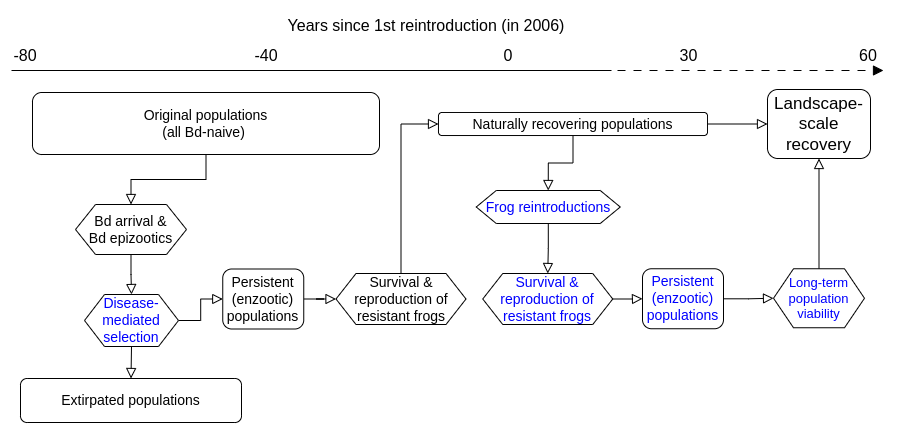
\includegraphics{figures/conceptual_model.png}

}

\caption{\label{fig-recovery-model}For MYL frogs, a conceptual model
depicting the Bd-caused decline and subsequent natural recovery (black
text), facilitated recovery via reintroductions, and the linkages
between these two pathways. Rectangles and hexagons represent outcomes
and processes, respectively. Blue text indicates components that are
included in the current study. The timeline shows the general sequence
of the components, with the dotted portion indicating a projection into
the future.}

\end{figure}

\newpage

\begin{figure}

{\centering 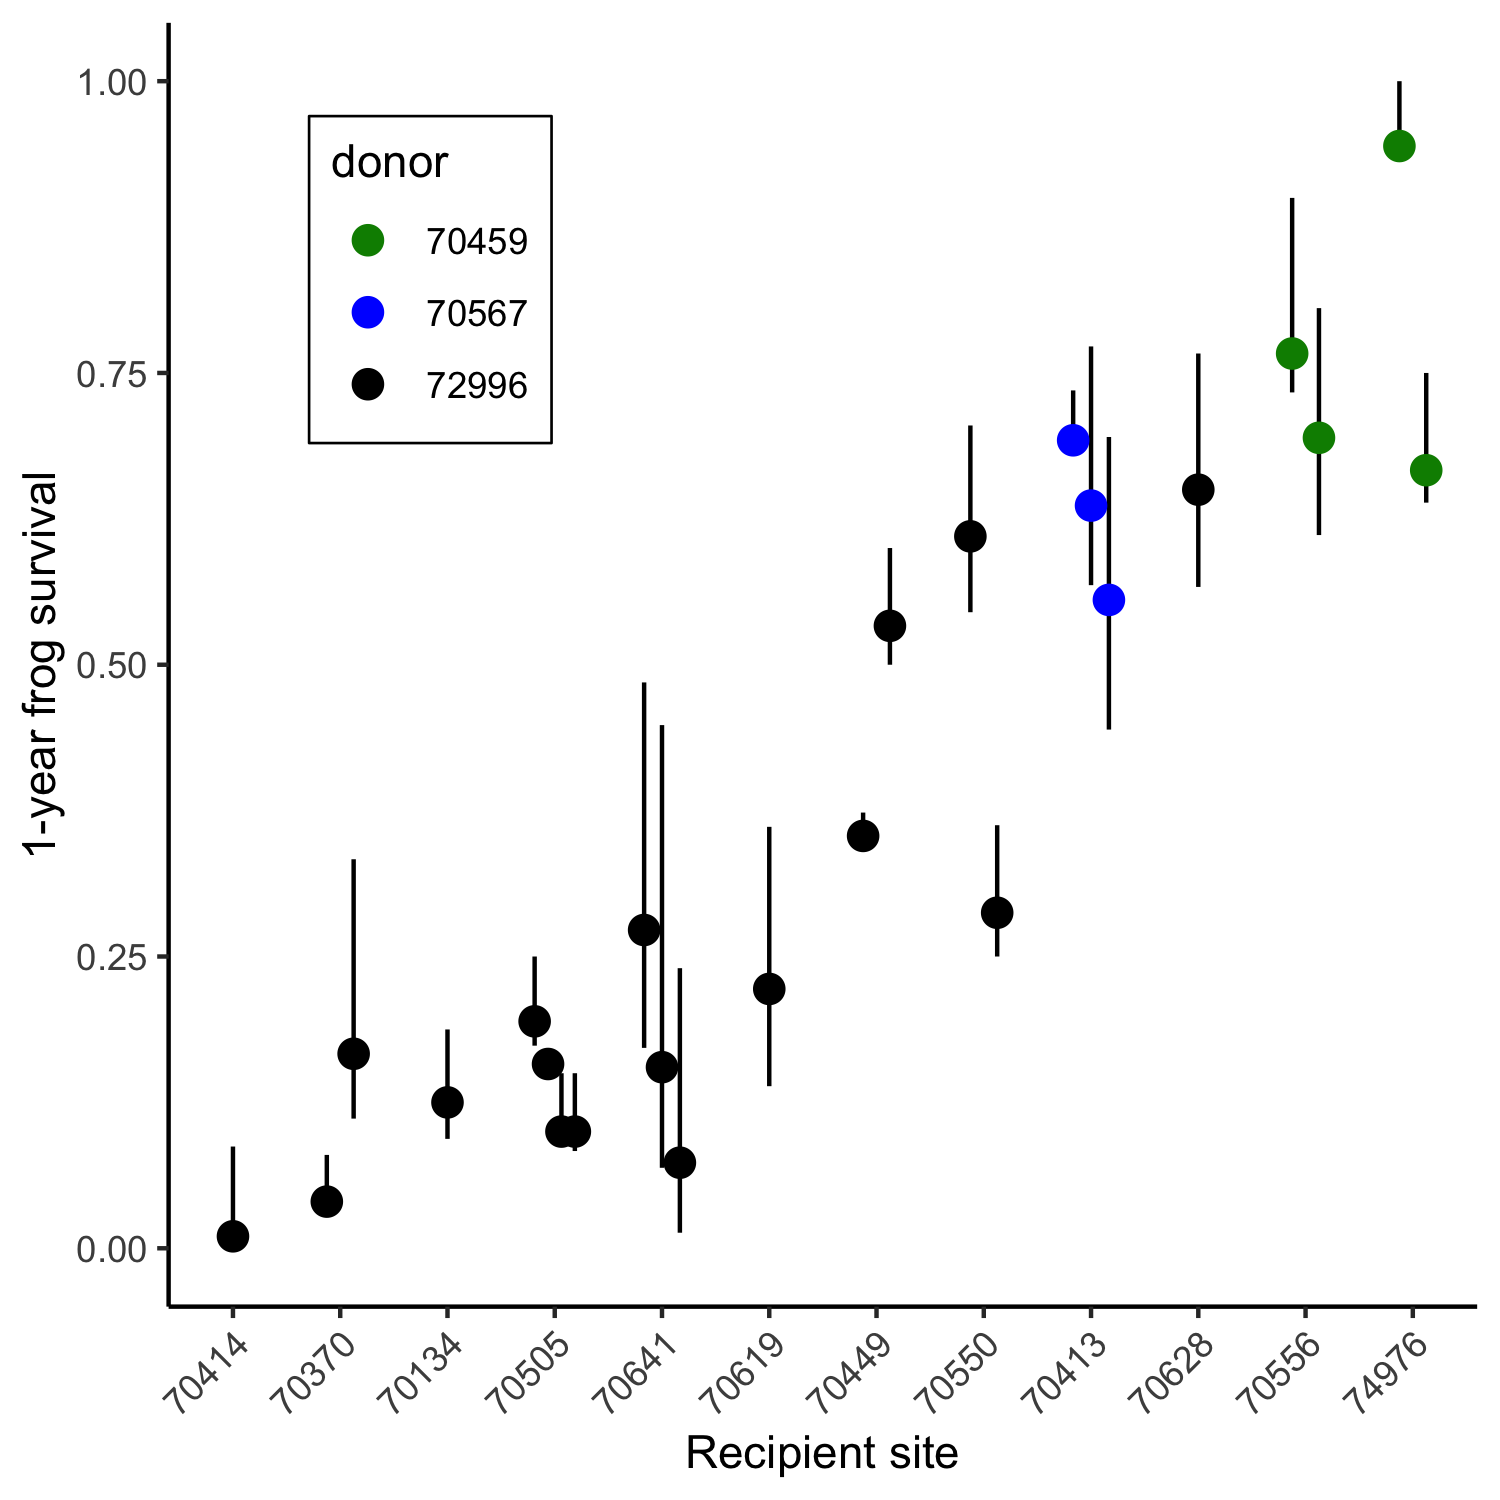
\includegraphics[width=4.6875in,height=\textheight]{figures/translocation_survival_bysiteid.png}

}

\caption{\label{fig-translocation-survival}Median 1-year survival for
each cohort of translocated frogs at the 12 recipient sites, as
estimated for each site from the mrmr CMR model. Error bars show the
95\% uncertainty intervals. Sites are arranged along the x-axis using
the average of the median 1-year survival per translocation at each
site. Dot colors indicate the donor population from which frogs in each
translocated cohort were collected. When multiple translocations were
conducted to a site, points and error bars are slightly offset to avoid
overlap.}

\end{figure}

\newpage

\begin{figure}

{\centering 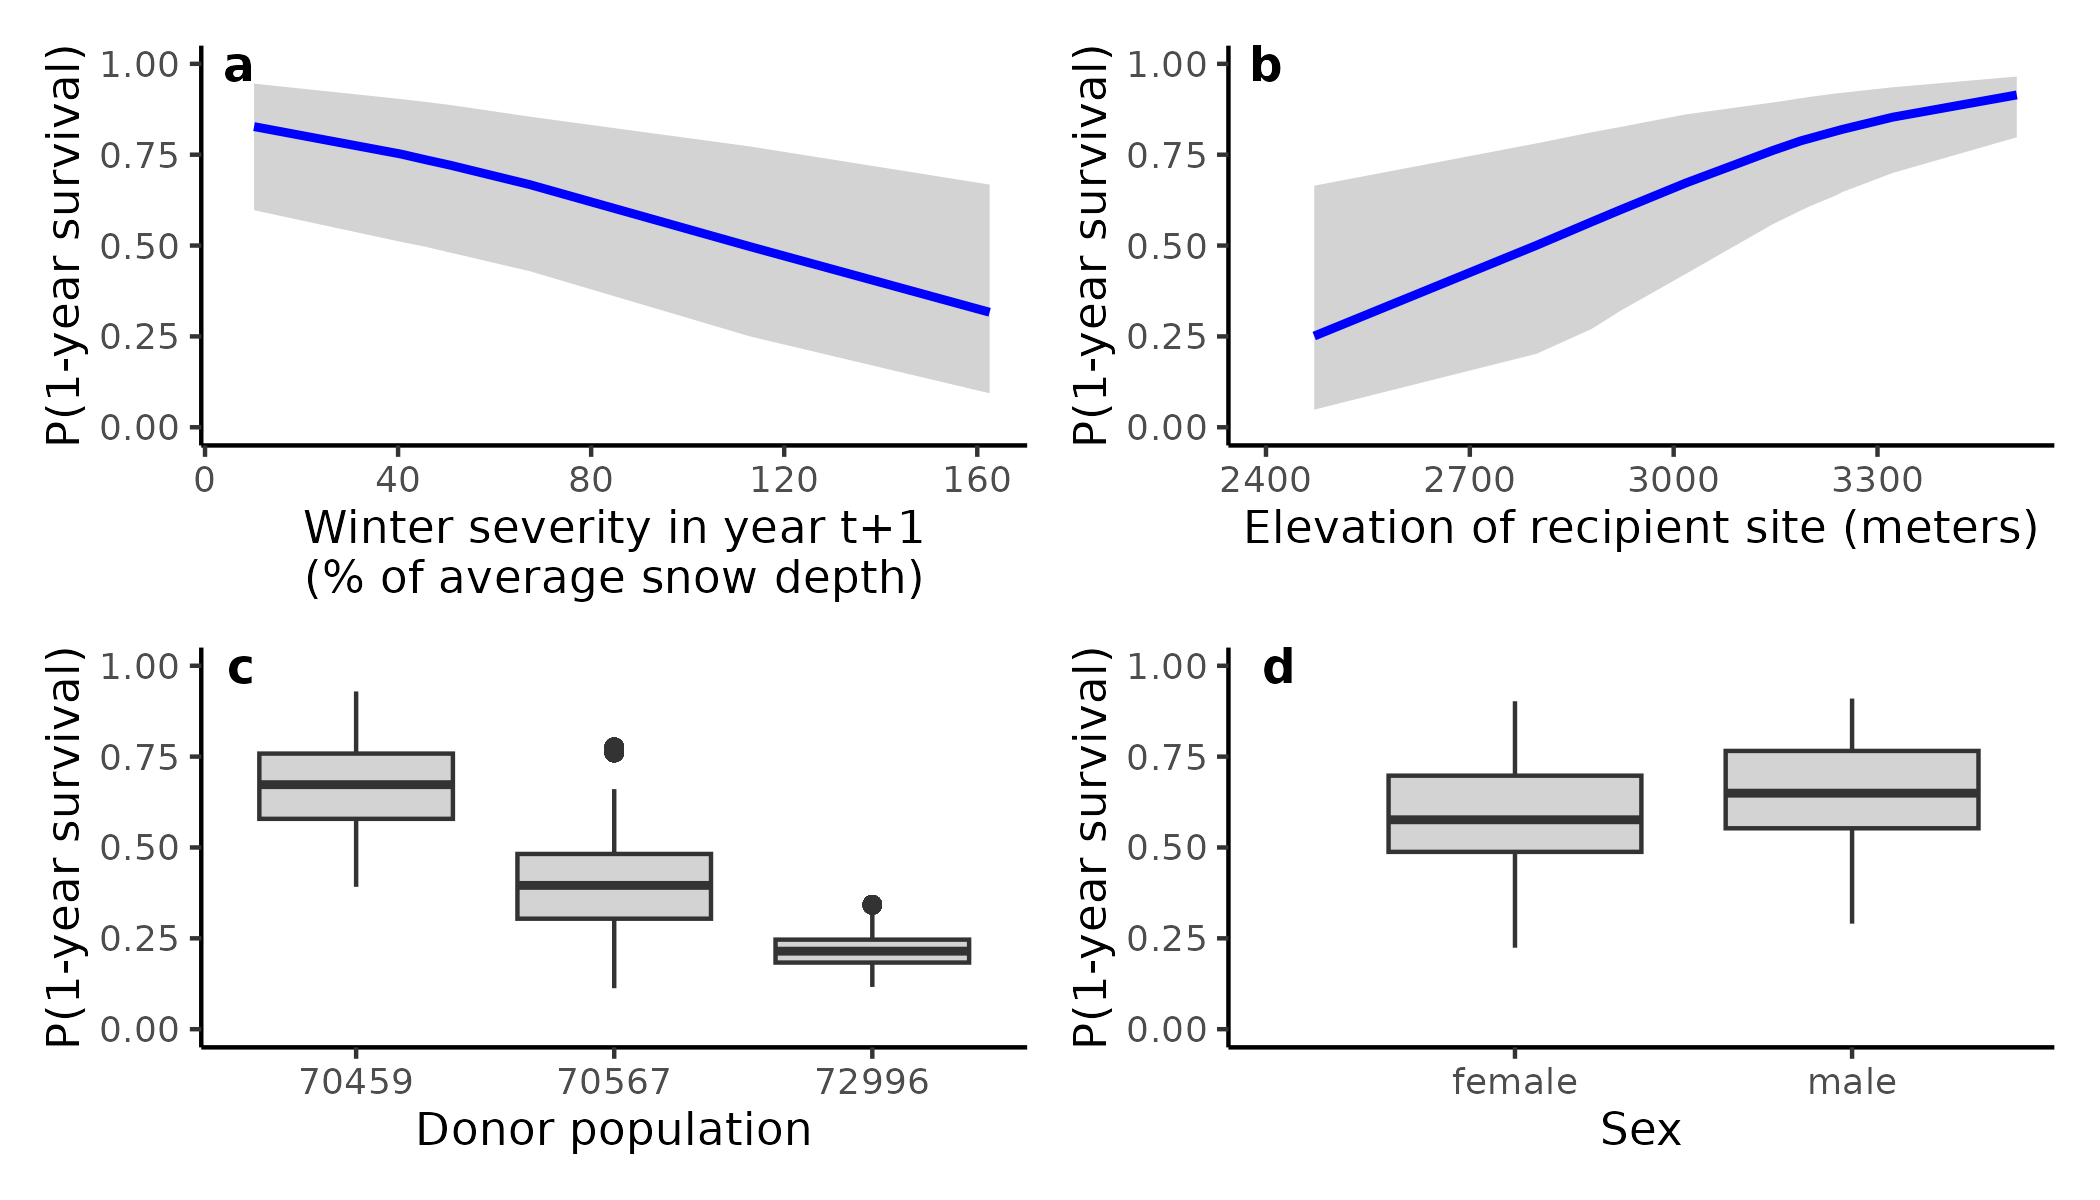
\includegraphics[width=5.72917in,height=\textheight]{figures/cond_effects_plot.png}

}

\caption{\label{fig-cond-effects}Results from the among-site
meta-analysis showing conditional effects of the important predictors of
1-year frog survival (expressed as a probability): (A) winter severity
in the year following translocation, (B) elevation of recipient site,
(C) donor population, and (D) sex. In (A) and (B), blue lines are
medians and gray ribbons are 95\% uncertainty intervals. In (C) and (D),
box plots show medians, first and third quartiles, largest and smallest
values within 1.5x interquartile range, and values outside the 1.5x
interquartile range.}

\end{figure}

\newpage

\begin{figure}

{\centering 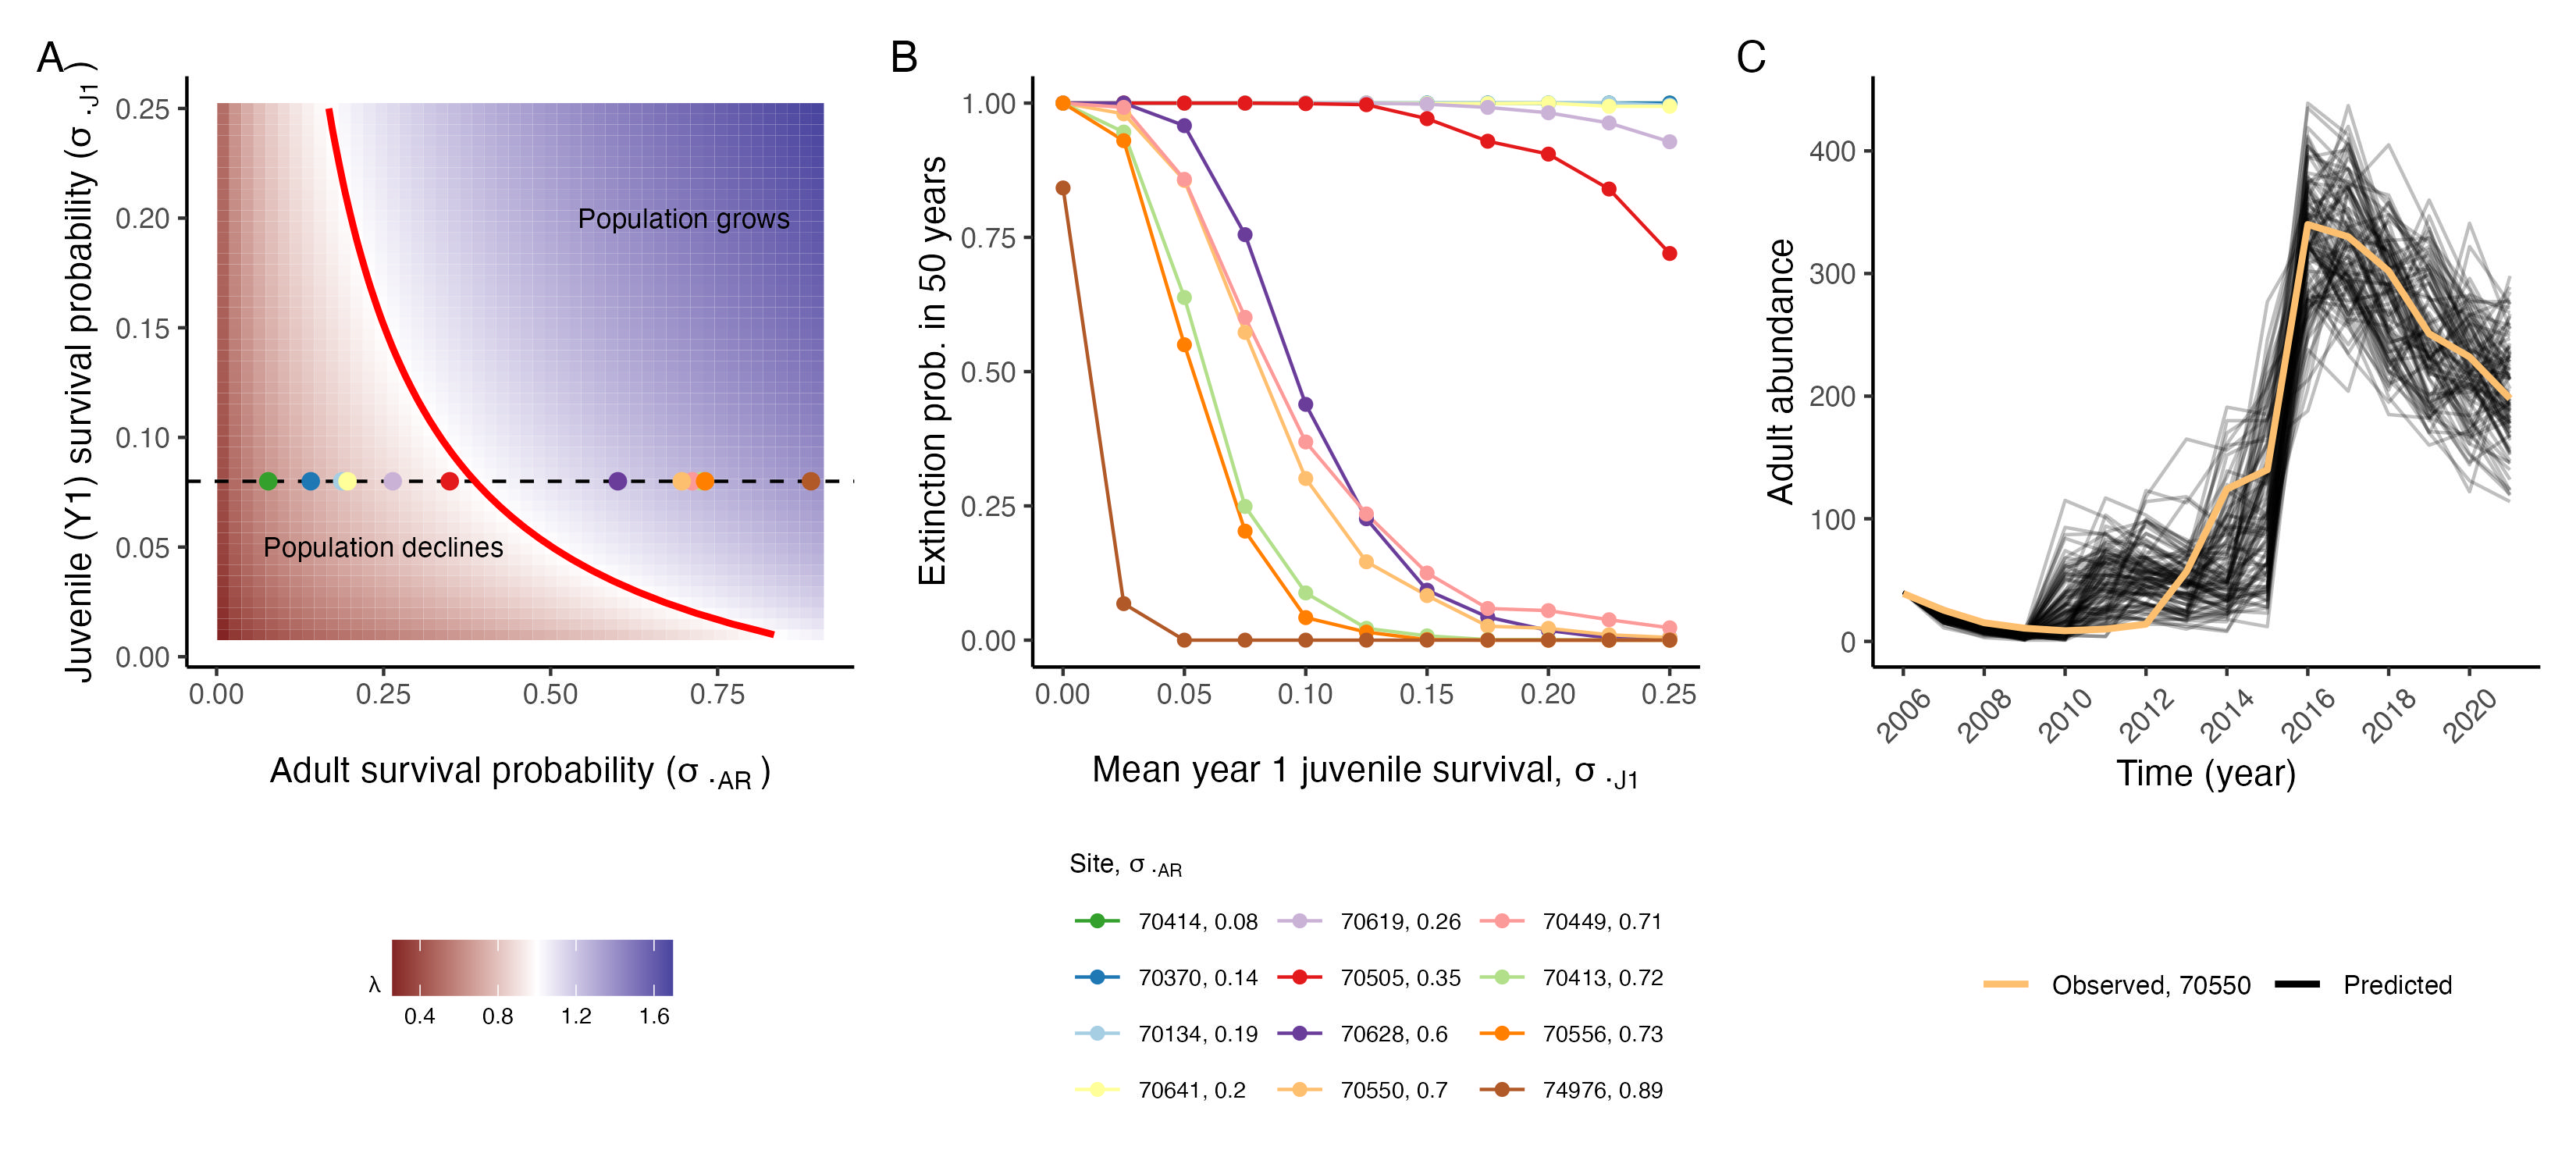
\includegraphics[width=6.77083in,height=\textheight]{figures/pop_viability_figures_for_manuscript.jpg}

}

\caption{\label{fig-viability}Results from population viability
analysis: (A) Predicted long-run growth rate \(\lambda\) for different
values of yearly adult survival probability \(\sigma_{A_R}\) and year-1
juvenile survival and recruitment probability \(\sigma_{J_1}\), given
the parameterized, deterministic model. Colored points show the
predicted \(\lambda\) values for the twelve translocated populations
when year-1 juvenile survival probability is \(\sigma_{J_1} = 0.09\)
(indicated by the dashed line). The red line shows where
\(\lambda = 1\). Note that the point for 70413 is mostly hidden behind
other points. (B) Predicted 50-year extinction probabilities of the 12
translocated populations, given demographic stochasticity, environmental
variability in \(\sigma_{J_1}\), and different mean values of
\(\sigma_{J_1}\). There are 6 lines at extinction probability = 1, 5 of
which (70414--70619) are hidden beneath the line for 70505 when
\(\sigma_{J_1} < 0.10\). (C) 100 simulated trajectories (black lines)
from the population viability model that most closely matched the
observed abundance trajectory of adult amphibians at site 70550 (light
orange).}

\end{figure}

\newpage

\begin{figure}

{\centering 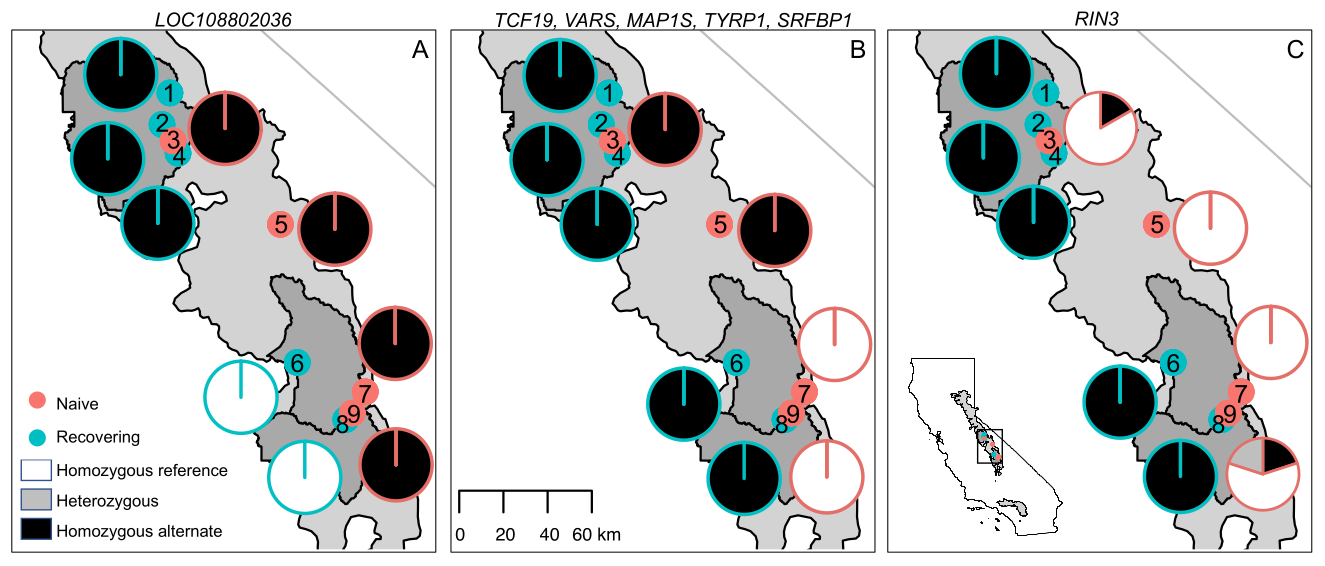
\includegraphics[width=6.25in,height=\textheight]{figures/allele_maps.png}

}

\caption{\label{fig-allelefrequencies}Evidence for selection on
individual variants in recovering MYL frog populations at the landscape
scale. For each of the 9 naive and recovering MYL frog populations
(indicated by numbered points), adjacent pie charts show allele
frequencies for the 11 outlier SNPs from 7 distinct genes: (A)
LOC108802036, (B) TCF19, VARS, MAP1S, TYRP1, and SRFBP1, and (C) RIN3.
Charts are superimposed on a map of the Sierra Nevada study area, with
Yosemite, Kings Canyon, and Sequoia National Parks (from north to south)
shown in dark gray, and the range boundary for MYL frogs shown in light
gray. The inset map locates the study area and range boundary in
California. Sites 1 and 4 (site id = 72996 and 70567, respectively) were
also used as sources of frogs in the frog population recovery study.}

\end{figure}

\newpage

\begin{figure}

{\centering 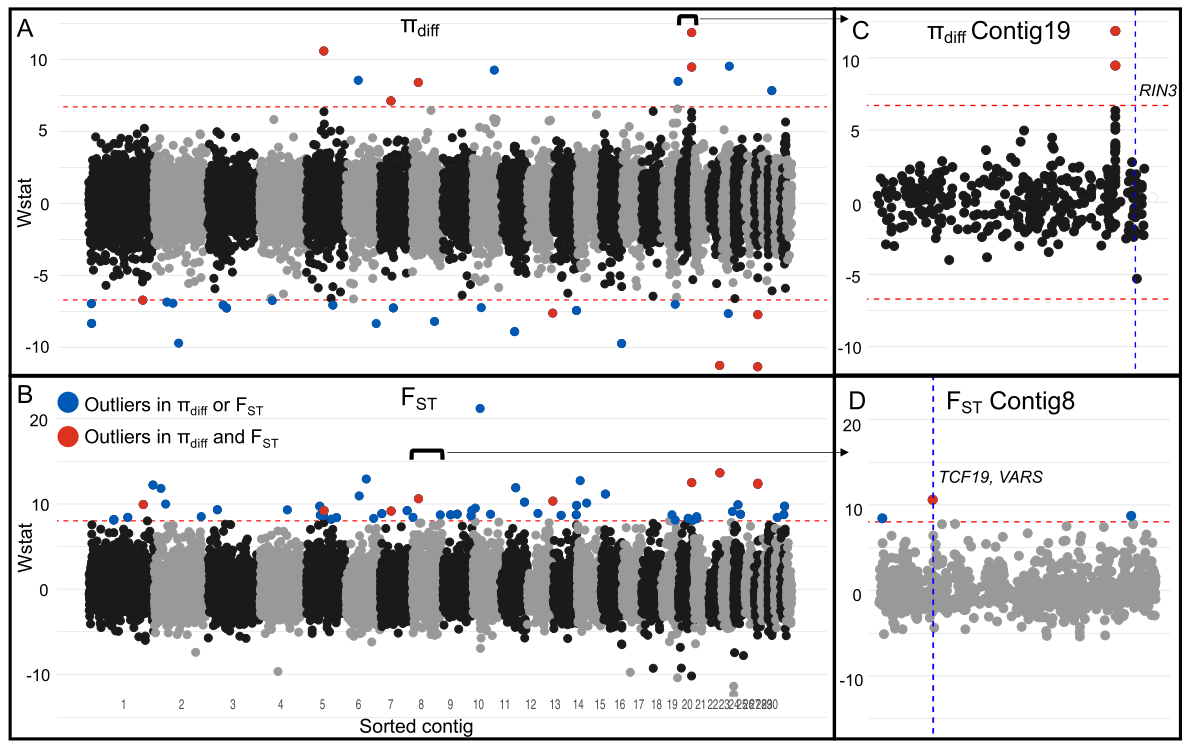
\includegraphics[width=5.72917in,height=\textheight]{figures/splinewindow_manhattan.png}

}

\caption{\label{fig-spline-manhattan}Evidence for selection on genomic
regions in recovering MYL frog populations. Manhattan plot of the
results from the splined window analysis showing outlier regions for the
difference in (A) nucleotide diversity \(\pi_{diff}\) and (B)
\emph{F\textsubscript{ST}}. In (A), outlier regions are shown above the
upper red dashed line and below the lower red dashed line. In (B),
outlier regions are shown above the single dashed red line. Outlier
regions for either \(\pi_{diff}\) or \emph{F\textsubscript{ST}} are
shown in blue and outlier regions for both \(\pi_{diff}\) and
\emph{F\textsubscript{ST}} are shown in red. (C) Magnified Contig19 from
(A) showing two adjacent outlier regions for \(\pi_{diff}\) 12.9Mb
upstream of the RIN3 outlier SNP (indicated with a dashed vertical blue
line). (D) Magnified Contig8 from from (B) showing the
\emph{F\textsubscript{ST}} outlier region that includes the outlier SNPs
TCF19 and VARS. This region of the genome contains 8 annotated genes
known to occur in the extended MHC Class I and III regions.}

\end{figure}

\newpage

\hypertarget{supporting-information}{%
\subsection{Supporting Information}\label{supporting-information}}

\hypertarget{frog-population-recovery-2}{%
\subsubsection{Frog population
recovery}\label{frog-population-recovery-2}}

\hypertarget{laboratory-methods}{%
\paragraph{Laboratory methods}\label{laboratory-methods}}

Swab extracts were analyzed using standard Bd DNA extraction and qPCR
methods \citep{boyle2004}, and extracts were analyzed singly instead of
in triplicate \citep{kriger2006}. For analysis of swabs collected during
2005--2014, we used standards developed from known concentrations of
zoospores \citep{boyle2004}, and after 2014, we used standards based on
single ITS1 PCR amplicons \citep{longo2013}. Based on paired comparisons
between samples analyzed using both types of standards, Bd in the study
area has an average of 60 ITS1 copies per zoospore. To express all qPCR
results as the number of ITS1 copies, starting quantities obtained using
the zoospore standard (measured as ``zoospore equivalents'') were
multiplied by 60. In addition, all qPCR quantities (regardless of
standard) were multiplied by 80 to account for the fact that DNA
extracts from swabs were diluted 80-fold during extraction and PCR
\citep{vredenburg2010}.

\hypertarget{cmr-model-structure}{%
\paragraph{CMR model structure}\label{cmr-model-structure}}

We estimated survival and recruitment for each site using open
population CMR models based on \citet{joseph2018}. For each individual
\(i=1, ..., M\) on each survey \(j=1, ..., n_j\): \(o_{i, j} = 1\) if
the individual was not detected, and \(o_{i, j}=2\) if the individual
was detected. Capture histories of \(M\) individuals are modeled,
although only \(N_s\) individuals were captured. This parameter expanded
data augmentation allows us to capture the possibility that undetected
individuals may have recruited into the adult population
\citep{royle2012}. Here, \(M\) was chosen to be three times the number
of observed individuals (\(3N_s\)) to be considerably greater than our
prior guess of \(N_s\).

We denote the true state of individual \(i\) as \(u_{i, t}\) for primary
period \(t = 1,..., n_t\). The four states that we consider are:
\(u_{i, t} = 1\) for individuals that have not recruited,
\(u_{i, t} =2\) for live adults, and \(u_{i, t} = 3\) for dead adults.
Each survey \(j=1, ..., n_j\) occurs in one of the \(n_t\) primary
periods, and we denote the primary period in which survey \(j\) takes
place as \(t_j\). Each primary period \(t\) occurs within one year, but
within a year there can be multiple primary periods. We set the year
containing the first primary period to \(y_{t = 1} = 1\), and generally
\(y_t\) represents the year containing primary period \(t\). Years
increment by one until the final year of the mark recapture efforts,
which we denote \(n_y\): \(y \in \{1, 2, ..., n_y\}\). We assume that
within a primary period, the state of each individual does not change
(i.e., individuals do not recruit into the adult population, gain or
lose Bd infection, or die). This assumption is justified by the short
time intervals between surveys within primary periods, in cases where
primary periods contain multiple secondary periods.

Live individuals are detected with probability \(p_j\), which is modeled
as:

\[p_j = \text{logit}^{-1}(X_j^{(p)} \beta^{(p)}),\]

where \(X_j^{(p)}\) is a known row vector and \(\beta^{(p)}\) an unknown
parameter vector. Not recruited and dead individuals are never captured.
We bundle these assumptions about the observation probabilities for
survey \(j\) into an emission matrix \(\Omega_j\):

\[
\Omega_j =
\begin{blockarray}{ccc}
  \text{Not detected} & \text{Detected} \\
\begin{block}{(cc)c}
  1 & 0 & \text{Not recruited} \\
  1 - p_j & p_j & \text{Alive} \\
  1 & 0 & \text{Dead} \\
\end{block}
\end{blockarray}
\]

The state transition matrix \(\Psi_{t, i}\) contains the probabilities
of individual \(i\) transitioning from state \(u_{i, t}\) (rows) to
\(u_{i, t+1}\) (columns) between primary period \(t\) and \(t+1\). For
non-introduced (i.e., naturally recruited) individuals, this matrix is
given by:

\[
\Psi_{t, i} =
\begin{blockarray}{cccc}
  \text{Not recruited} & \text{Alive} & \text{Dead} \\
\begin{block}{(ccc)c}
  1 - \lambda_t & \lambda_t & 0 & \text{Not recruited} \\
  0 & \phi_t & 1 - \phi_t & \text{Alive} \\
  0 & 1 & 1 & \text{Dead} \\
\end{block}
\end{blockarray},
\] where \(\lambda_t\) is the probability of recruiting in time \(t\)
and \(\phi_t\) is the probability of survival in time \(t\).

For introduced individuals, which have deterministic recruitment (i.e.,
they recruit when introduced), the state transition matrix is given by:

\[
\Psi_{t, i} =
\begin{blockarray}{cccc}
  \text{Not recruited} & \text{Alive} & \text{Dead} \\
\begin{block}{(ccc)c}
  1 - I_{t, i} & I_{t, i} & 0 & \text{Not recruited} \\
  0 & \phi_t & 1 - \phi_t & \text{Alive} \\
  0 & 1 & 1 & \text{Dead} \\
\end{block}
\end{blockarray},
\] where \(I_{t, i}\) is a known indicator function for whether
individual \(i\) was introduced in primary period \(t\).

We allow recruitment probabilities to vary in time via random effects,
such that:

\[\lambda_t = \text{logit}^{-1}(\alpha^{(\lambda)} + \epsilon^{(\lambda)}_t),\]

where \(\alpha^{(\lambda)}\) is an intercept parameter and
\(\epsilon^{(\lambda)}_t\) is an adjustment for time \(t\).

Survival probabilities also vary in time, and as a function of known
covariates:

\[\phi_t = \text{logit}^{-1}(X^{(\phi)}_t \beta^{(\phi)} + \epsilon^{(\phi)}_t),\]

where \(X^{(\phi)}_t\) is a row vector of known covariates,
\(\beta^{(\phi)}\) is a column vector of unknown coefficients, and
\(\epsilon^{(\phi)}_t\) is an adjustment for time \(t\).

To complete the specification of the Bayesian model, we specify priors
for all unknown parameters. The recruitment parameter priors were
specified as follows:

\[\alpha^{(\lambda)} \sim N(0,1),\]
\[\sigma^{(\lambda)} \sim N_+(0,1),\]
\[\epsilon^{(\lambda)}_t \sim N(0, \sigma^{(\lambda)}),\] for periods
\(t=1, ..., T\). Here \(N\) represents the normal distribution and
\(N_+\) the half normal distribution with positive support.

Survival parameter priors were specified similarly as:

\[\beta^{(\phi)} \sim N(0, 1),\] \[\sigma^{(\phi)} \sim N_+(0, 1),\]
\[\epsilon^{(\phi)}_t \sim N(0, \sigma^{(\phi)}),\] for time
\(t=1, ..., T\).

The detection model coefficient vector also received a standard normal
prior \(\beta^{(p)} \sim N(0, 1)\).

We computed the likelihood of each individual capture history using the
forward algorithm, and we estimated the latent states using the
forward-backward algorithm \citep{zucchini2009, joseph2018}.

All of the code to specify and fit the model in Stan is available in the
open source mrmr package \citep{joseph2019}.

The joint distribution of the resulting model can be written as follows:

\begin{multline*}
[\alpha^{(\lambda)}, \sigma^{(\lambda)}, \epsilon^{(\lambda)}_{1:T}, \beta^{(\phi)}, \sigma^{(\phi)}, \epsilon^{(\phi)}_{1:T}, \beta^{(p)} \mid \pmb Y] \propto \prod_{i=1}^M [Y_i \mid \alpha^{(\lambda)}, \epsilon^{(\lambda)}_{1:T}, \beta^{(\phi)}, \epsilon^{(\phi)}_{1:T}, \beta^{(p)}] \times \\
\prod_{t=1}^T [\epsilon_t^{(\lambda)} \mid \sigma^{(\lambda)}] [\epsilon_t^{(\phi])} \mid \sigma^{(\phi)}] [\sigma^{(\lambda)}] [\sigma^{(\phi)}] [\alpha^{(\lambda)}] [\beta^{(\phi)}] [\beta^{(p)}],
\end{multline*}

where \(\pmb Y\) is an \(M \times T\) detection matrix, and \(Y_i\) the
capture history of individual \(i\).

\hypertarget{among-site-survival-modeling}{%
\paragraph{Among-site survival
modeling}\label{among-site-survival-modeling}}

The objective of this analysis is to describe the influence of site,
cohort, and individual level characteristics on post-translocation frog
survival. By modeling survival estimates obtained from site-specific
mrmr CMR analyses, we are in effect conducting an among-site
meta-analysis. Although it would theoretically be possible to estimate
survival covariate effects in a joint CMR model that integrates capture
histories across all sites, this was impractical due to computational
requirements of the CMR models (namely, run time and memory).

We used Bayesian generalized linear mixed models to investigate
predictors of survival among sites. The response \(y_i\) is binary,
representing a point estimate of whether individual \(i\) survived in
the year following translocation. We generated these point estimates by
rounding the posterior median of 1-year post-introduction survival for
each individual (from site-specific mrmr CMR models) and modeled the
data using a Bernoulli distribution:

\[y_i \sim \text{Bernoulli}(p_i),\]

where \(p_i\) is the probability of survival.

We modeled variation in probabilities as follows:

\[\text{logit}(p_i) = \alpha + X_i \pmb \beta + \pmb \nu_{g[1:N]},\]

where \(\alpha\) is an intercept, \(X_i\) is a length \(K\) row vector
of predictors, \(\pmb \beta\) is a column vector of predictor effects,
and \(\pmb \nu\) a vector of group level random effects. Here \(g[i]\)
refers to the group \(g\) containing individual \(i\), and we estimate
an adjustment for each of the \(G\) groups (\(\nu_1, ..., \nu_G\)).

These models were fit using the \texttt{stan\_glmer()} function in the
rstanarm package, with default priors described below
\citep{rstanarm2022}. These priors are vague, but include data-dependent
scaling as follows to account for different input variable scales.
However, because we standardized all predictor variables similarly to
have equal variance (by centering and dividing by twice the sample
standard deviation), the resulting priors are identical. Specifically,
we have:

\[\alpha \sim \text{Normal}(0, 2.5),\] and

\[\beta_k \sim \text{Normal}(0, 5),\]

for \(k=1, ..., K\) where \(K\) is the number of predictor variables.

The default prior for group level adjustments \(\nu_1, ..., \nu_G\) in
rstanarm is a zero-mean Gaussian, where the covariance matrix is
constructed from a correlation matrix with an LKJ prior, and a vector of
variance parameters -- the decomposition of variance prior with unit
regularization, concentration, shape, and scale parameters
\citep{lewandowski2009}.

We drew posterior samples using Dynamic Hamiltonian Monte Carlo in Stan,
with four parallel chains, each run for 10,000 iterations, discarding
the first half of each chain as warm-up draws \citep{rstanarm2022}. We
used Rhat statistics and trace plots to verify convergence. We
considered models with different subsets of fixed and random effects,
and used approximate leave-one-out cross validation to identify the best
model \citep{vehtari2016}.

\hypertarget{population-viability-modeling-1}{%
\subsubsection{Population viability
modeling}\label{population-viability-modeling-1}}

\hypertarget{incorporating-yearly-variability-in-vital-rates}{%
\paragraph{Incorporating yearly variability in vital
rates}\label{incorporating-yearly-variability-in-vital-rates}}

We computed yearly survival probabilities for translocated adults
\(\sigma_{A_T}\) and naturally recruited adults \(\sigma_{A_R}\) from
the posterior distribution of individual state trajectories derived from
mrmr CMR models. Although we observed yearly variability in adult
survival within a population, the magnitude of this variability was
small compared to among-population variability
(Figure~\ref{fig-translocation-survival}). Thus, we did not include
yearly within-population variability in adult survival in this analysis.
However, within a population there was substantial yearly variability in
the successful recruitment of adults, greater than what we would expect
from Poisson variability around a mean value. Therefore, we allowed for
yearly variability in the probability of year-1 juvenile survival and
recruitment (additional details provided in \textbf{Estimating model
parameters} below). We also could have included environmental
stochasticity in year-2 juvenile survival and recruitment
\(\sigma_{J_2}\), but our elasticity analysis (\textbf{Supporting
Information - Population viability modeling - Model analysis and
simulation}) showed that this parameter had little effect on host growth
rate relative to \(\sigma_{J_1}\) (Figure~\ref{fig-viability-supp} SI).

\hypertarget{estimating-model-parameters}{%
\paragraph{Estimating model
parameters}\label{estimating-model-parameters}}

The baseline parameter values for the model and how they were estimated
are given in Table~\ref{tbl-param_values}. Parameters \(\sigma_{A_T}\)
and \(\sigma_{A_R}\) were extracted directly from our CMR models (see
\textbf{Materials and Methods - Frog populaton recovery - Estimation of
frog survival and abundance} and \textbf{Supporting Information - Frog
population recovery - CMR model structure} for details). For populations
where we had a sufficient number of PIT-tagged, naturally-recruited
adults, we observed that \(\sigma_{A_T}\) and \(\sigma_{A_R}\) could be
notably different, with \(\sigma_{A_R} > \sigma_{A_T}\)
(Figure~\ref{fig-compare_surv_probs} SI). For populations lacking
sufficient numbers of naturally-recruited adults, we were unable to
directly estimate \(\sigma_{A_R}\), and instead set
\(\sigma_{A_R} = \sigma_{A_T}\).

To estimate the \(\sigma_{A_R}\), we used the posterior distribution of
predicted true states for naturally-recruited individuals (1=not
recruited, 2=alive, 3=dead, as described in \textbf{Supporting
Information - Frog population recovery - CMR model structure}), then
calculated the posterior probability of individuals surviving between
consecutive primary periods, conditional on being alive in the first
primary period (e.g., given a value of 2 (alive) in the first primary
period, how often was the value still 2 (alive) in the next primary
period compared to 3 (dead)?) . This yielded posterior distributions for
survival probabilities between primary periods. However, because the
time interval between primary periods differed, the survival
probabilities between different consecutive primary periods were not
directly comparable. To address this, we converted the survival
probabilities between each consecutive primary period to per day death
rates, propagating the uncertainty from the posterior distributions. We
then took a weighted average of these death rates, weighted by the time
interval between primary periods, to get the average per day death rate
over the entire CMR survey. We converted this per day death rate \(d\)
back to a yearly survival probability using
\(\exp(-d \times 365 \text{ days})\). We used the same procedure for
\(\sigma_{A_T}\) such that our estimates of average yearly survival
probability were comparable between \(\sigma_{A_R}\) and
\(\sigma_{A_T}\).

\hypertarget{model-analysis-and-simulation}{%
\paragraph{Model analysis and
simulation}\label{model-analysis-and-simulation}}

We performed four analyses on our model. First, we considered a
deterministic version of our model with no yearly heterogeneity in
year-1 juvenile survival and recruitment probability \(\sigma_{J_1}\),
and calculated the predicted long-run growth rate \(\lambda\) of a
population for different values of \(\sigma_{A_R}\) and
\(\sigma_{J_1}\). We then fixed \(\sigma_{J_1} = 0.09\) and calculated
the predicted growth rate of our 12 populations.

Second, we performed a local elasticity analysis on \(\lambda\) with
respect to parameters \(\sigma_{J_1}\), \(\sigma_{J_2}\),
\(\sigma_{A_R}\), and \(F\) to determine how small changes in these
parameters could influence the long-run deterministic growth rate of
populations (Figure~\ref{fig-viability-supp} SI).

Third, we defined a version of the model with demographic and
environmental stochasticity, where environmental stochasticity was
represented by among-year variability in \(\sigma_{J_1}\). We used this
model to simulate a one-time introduction of 40 translocated adult
frogs. We ran this simulation 1000 times for each population and
computed the probability of a population becoming extinct after 50 years
given the observed parameter values and environmental stochasticity in
\(\sigma_{J_1}\). We varied the mean recruitment probability
\(\sigma_{J_1}\) from 0 and 0.25 and drew values of \(\sigma_{J_1}\)
each year from a beta distribution with a dispersion parameter of
\(\phi = 2\) (when \(\sigma_{J_1} = 0.5\) and \(\phi = 2\) the beta
distribution is uniform between 0 and 1). Using different values of
\(\phi\) does not qualitatively change the existence of distinct
extinction dynamics between populations with \(\sigma_{A_R} < 0.5\) and
those with \(\sigma_{A_R} > 0.5\). However, increasing yearly
variability in \(\sigma_{J_1}\) increases extinction risk for all
populations. For example, if we set \(\phi = 0.001\), such that in a
given year essentially either all year-1 juveniles survive or all of
them die, populations with \(\sigma_{A_R} > 0.5\) need to have
\(\sigma_{J_1}\) greater than 0.2 to have a 50-year extinction
probability of less 50\%. Because we do not pit tag juveniles, we do not
have CMR estimates for \(\sigma_{J_1}\) or \(\phi\). However, based on
qualitative and semi-quantitative field observations over 25 years, a
value of \(\sigma_{J_1} = 0.25\) in the presence of Bd is probably a
reasonable estimate for many populations. Thus, we expect our model
predictions to be conservative with regards to population recovery.

Finally, we assessed whether our stochastic model could reproduce
observed trajectories of population recovery. We focused on population
70550 because this was our longest CMR time series for a translocated
population and because this population shows evidence of substantial
post-translocation increases in adult abundance associated with
population establishment and recovery. We simulated our model for 16
years, repeating the simulation 50,000 times. For each run and each
year, we drew \(\sigma_{J_1}\) from a uniform distribution between 0 and
1 (or equivalently a beta distribution with mean 0.5 and \(\phi = 2\)).
Using Approximate Bayesian Computing and rejection sampling
\citep{kosmala2016}, we identified the top 2\% of trajectories (i.e.,
1000 trajectories) that minimized the sum of squared errors between the
observed and predicted data. The yearly \(\sigma_{J_1}\) values
associated with these ``best'' trajectories represented an approximate
posterior distribution \citep{beaumont2010}. Using these best fit
trajectories, we assessed whether our model could qualitatively describe
the patterns of recovery in the observed data for population 70550.

\hypertarget{frog-evolution-in-response-to-bd-2}{%
\subsubsection{Frog evolution in response to
Bd}\label{frog-evolution-in-response-to-bd-2}}

\hypertarget{study-design}{%
\paragraph{Study design}\label{study-design}}

To gain insights into the role of evolution in the development of
resistance by MYL frogs, we compared frog exomes sampled in naive versus
recovering populations. Comparing populations with different infection
histories allowed larger sample sizes and replication across the
landscape. The alternative approach of comparing samples from the same
populations before and after Bd exposure isn't feasible in this system
because Bd arrived in most MYL frog populations decades ago and
population persistence/recovery is rare and unpredictable. As a result,
samples from recovering populations collected before and after Bd
exposure are not available and are unlikely to be available in the
future.

Our study design, in which we compared frog genomes in naive and
recovering populations, required sampling populations across the range
of MYL frogs in the southern Sierra Nevada. This is due to the fact that
very few MYL frog populations remain in the naive state, and those that
do are scattered across a wide latitudinal range, from Yosemite National
Park in the north to southern Kings Canyon National Park in south. To
minimize potential confounding effects caused by known variation in frog
genotypes across latitude \citep{byrne2023}, we selected sampling sites
such that both population types were represented across similar
latitudinal ranges (Figure~\ref{fig-allelefrequencies}).

\hypertarget{go-analysis}{%
\paragraph{GO analysis}\label{go-analysis}}

In \textbf{Results-Frog evolution in response to Bd}, we describe the
stringent set of outlier variants (identified using a
Bonferroni-corrected p-value of 0.01). A liberal set of outlier
variants, identified using a Bonferroni-corrected p-value of 0.05,
included 38 outliers (35 SNPs and 3 INDELS) from 30 distinct genes
across 16 contigs. We used this liberal set to determine if any GO
biological functions, molecular functions, or cellular processes were
overrepresented. To do this, we retrieved the BLAST hits and mapped GO
terms for each gene in our targeted transcriptome. We then conducted a
statistical overrepresentation test (Fisher's exact test) using Blast2GO
\citep{conesa2005} to compare the 30 unique outlier genes to the
complete set of genes in our target transcriptome. We repeated this
process for the set of 35 genes located in the 9 shared regions of the
\emph{F\textsubscript{ST}} and \(\pi_{diff}\) splined windows.

\hypertarget{genetic-diversity}{%
\paragraph{Genetic diversity}\label{genetic-diversity}}

To characterize general patterns of genetic diversity between naive and
recovering populations, we conducted three analyses. First, we
calculated heterozygosity for each sampled frog using VCFtools
\citep{danecek2011}. Second, to characterize genome-wide patterns of
diversity, we used VCFtools to calculate nucleotide diversity (\(\pi\))
in 100kb sliding windows along the genome for each population. Third, we
calculated average \(\pi\) per population within each of the 9 outlier
windows identified in the splined window analysis.

Average individual-level heterozygosity and genome-wide population-level
\(\pi\) were similar between the naive and recovering groups
(Figure~\ref{fig-violinplot-heterozy} SI;
Figure~\ref{fig-boxplot-genomewide-pi-by-pop} SI). Within each of the 9
outlier windows, average \(\pi\) shows considerable variation between
populations (Figure~\ref{fig-boxplot-pi-by-windowpop} SI) and no obvious
patterns between the naive and recovering groups.

\newpage

\hypertarget{figures-1}{%
\subsubsection{Figures}\label{figures-1}}

\newpage

\begin{figure}

{\centering 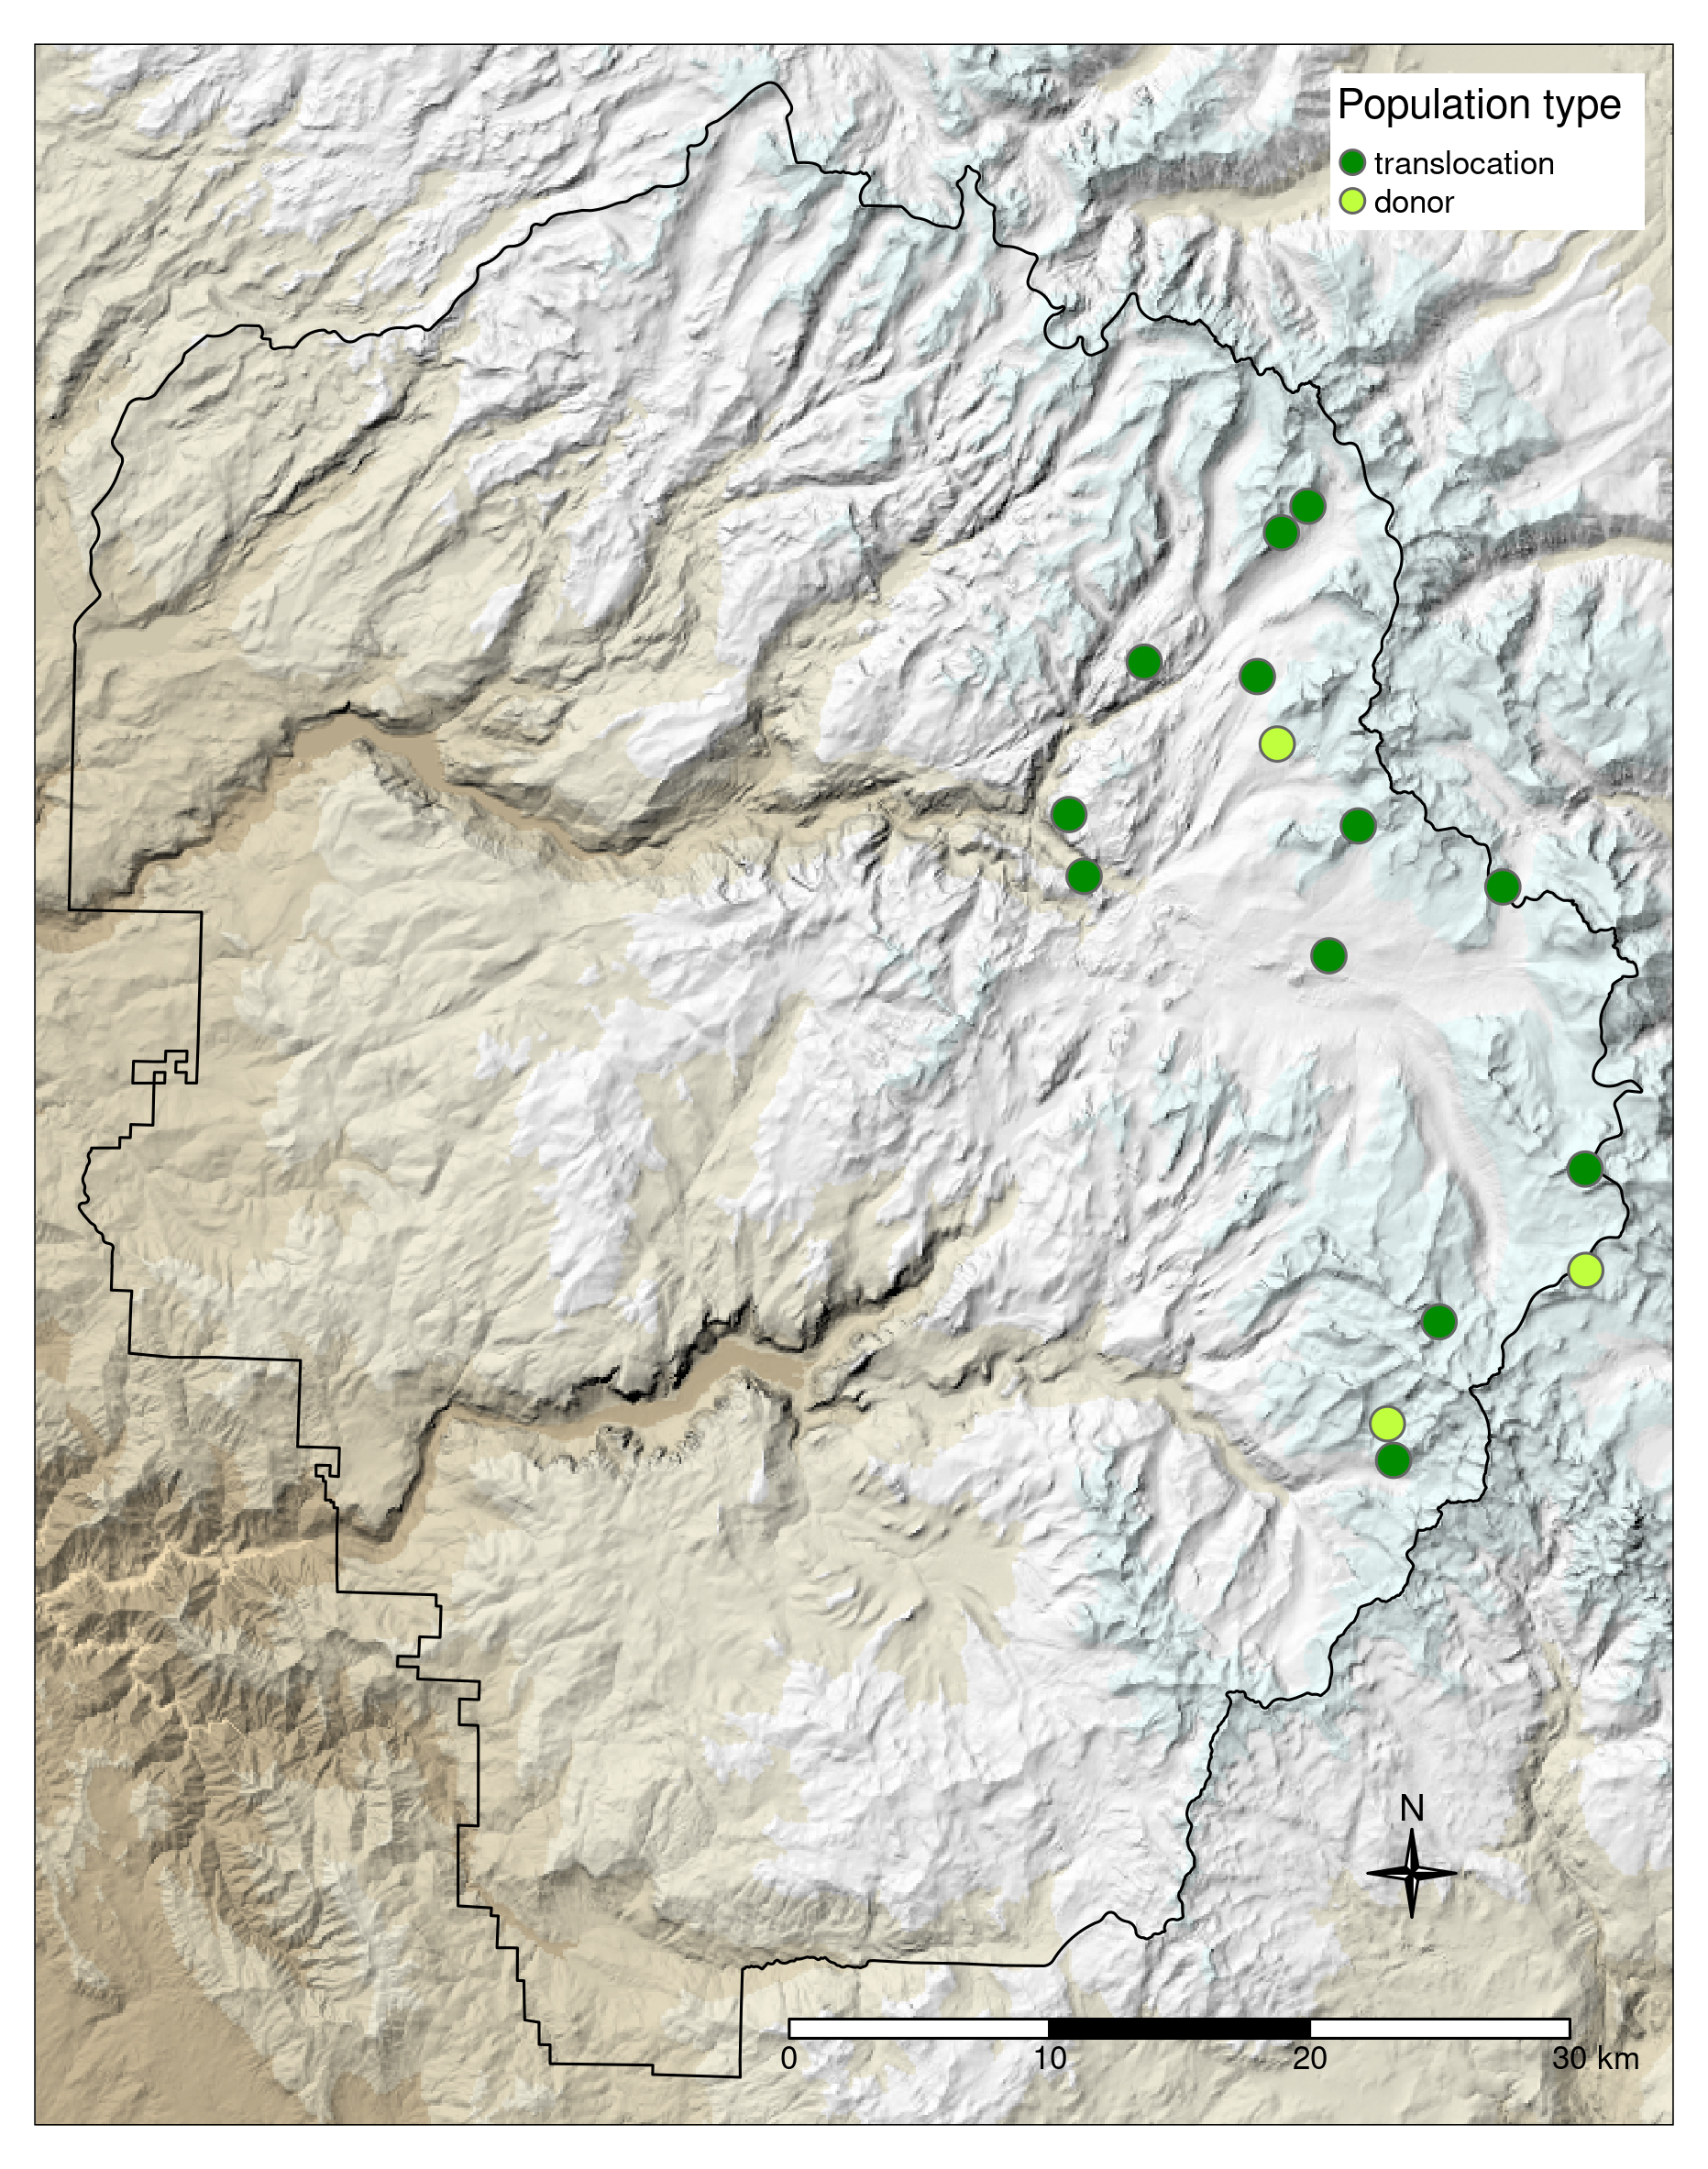
\includegraphics[width=4.16667in,height=\textheight]{figures/map_translocation_points.png}

}

\caption{\label{fig-yosemap}Map showing the locations of translocated
and donor MYL frog populations in Yosemite National Park (park boundary
indicated by gray polygon). Symbol shapes indicate the donor population
used for each translocation site, and 5-digit numbers identify each
donor and translocation site. To obscure the exact locations of
populations, random noise was added to all point coordinates. Inset map
shows the location of Yosemite within California. In both maps,
elevation is indicated by the colored hillshade layer (dark green =
lowest elevation, white = highest elevation).}

\end{figure}

\newpage

\begin{figure}

{\centering 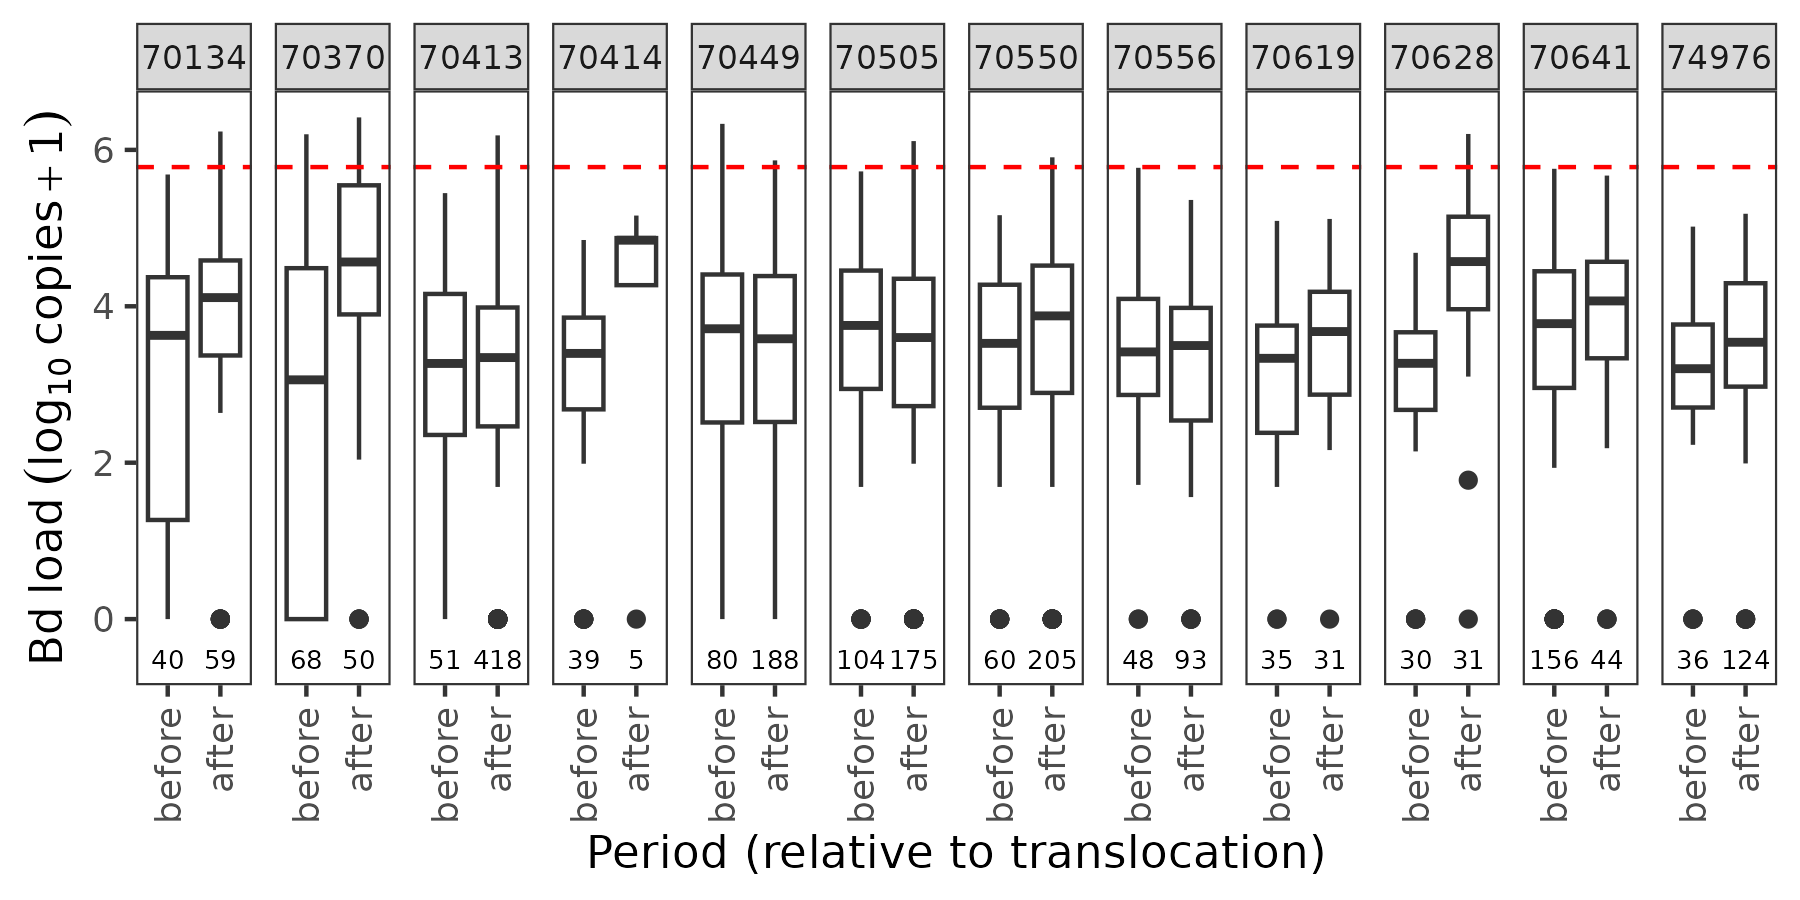
\includegraphics[width=6.5625in,height=\textheight]{figures/bdload_beforeafter.png}

}

\caption{\label{fig-bdload-beforeafter}For frogs translocated to each of
the 12 recipient sites, Bd loads for the period immediately prior to
translocation versus during the 1-year period after translocation. Bd
loads are expressed as the number of ITS1 copies per skin swab, as
estimated by qPCR of the Bd ITS1 region. Box plots show medians, first
and third quartiles, largest and smallest values within 1.5x
interquartile range, and values outside the 1.5x interquartile range.
Loads indicative of severe disease are \textgreater{} 5.8 ITS copies (on
a log\textsubscript{10} scale). Samples sizes are provided immediately
above the x-axis.}

\end{figure}

\newpage

\begin{figure}

{\centering 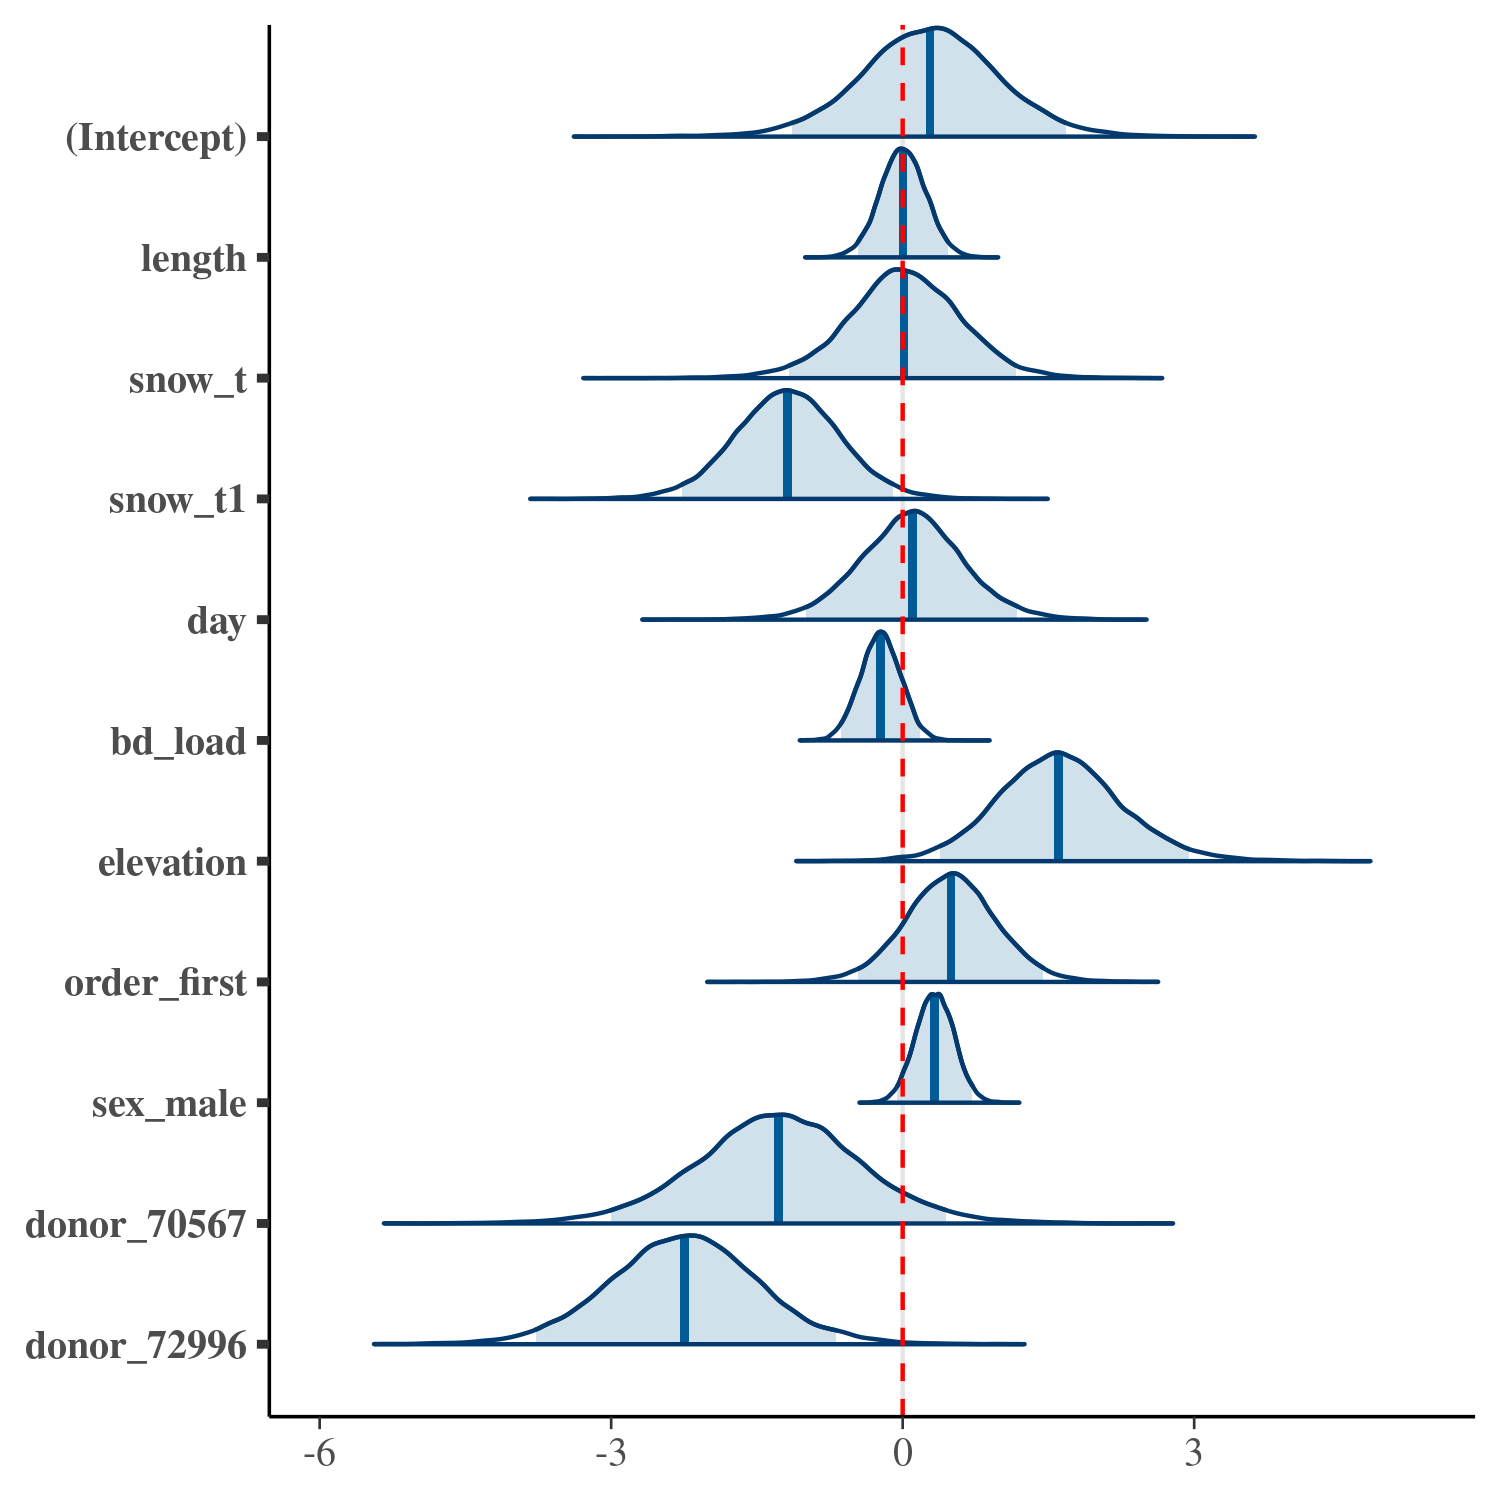
\includegraphics[width=5.20833in,height=\textheight]{figures/mcmc_areas_m1d.png}

}

\caption{\label{fig-survival-postdens}Results from the among-site
meta-analysis, showing that Bd load is not an important predictor of
post-translocation frog survival. Depicted distributions are the
estimated posterior density curves and shaded 95\% uncertainty intervals
for the intercept and all predictor variables from the best model. In
the Bayesian framework in which the model was developed, variables are
considered important predictors if the associated uncertainty interval
does not overlap zero (indicated by the dashed red line). Predictor
variables shown on the y-axis are defined as follows: length = frog
size, snow\_t = winter severity in the year of translocation (measured
on April 1), snow\_t1 = winter severity in the year following
translocation (measured on April 1), day = day of year on which a
translocation was conducted, bd\_load = Bd load, elevation = site
elevation, order\_first = within-site translocation order, sex\_male =
frog sex, donor\_70567 and donor\_72996 = donor population.}

\end{figure}

\newpage

\begin{figure}

{\centering 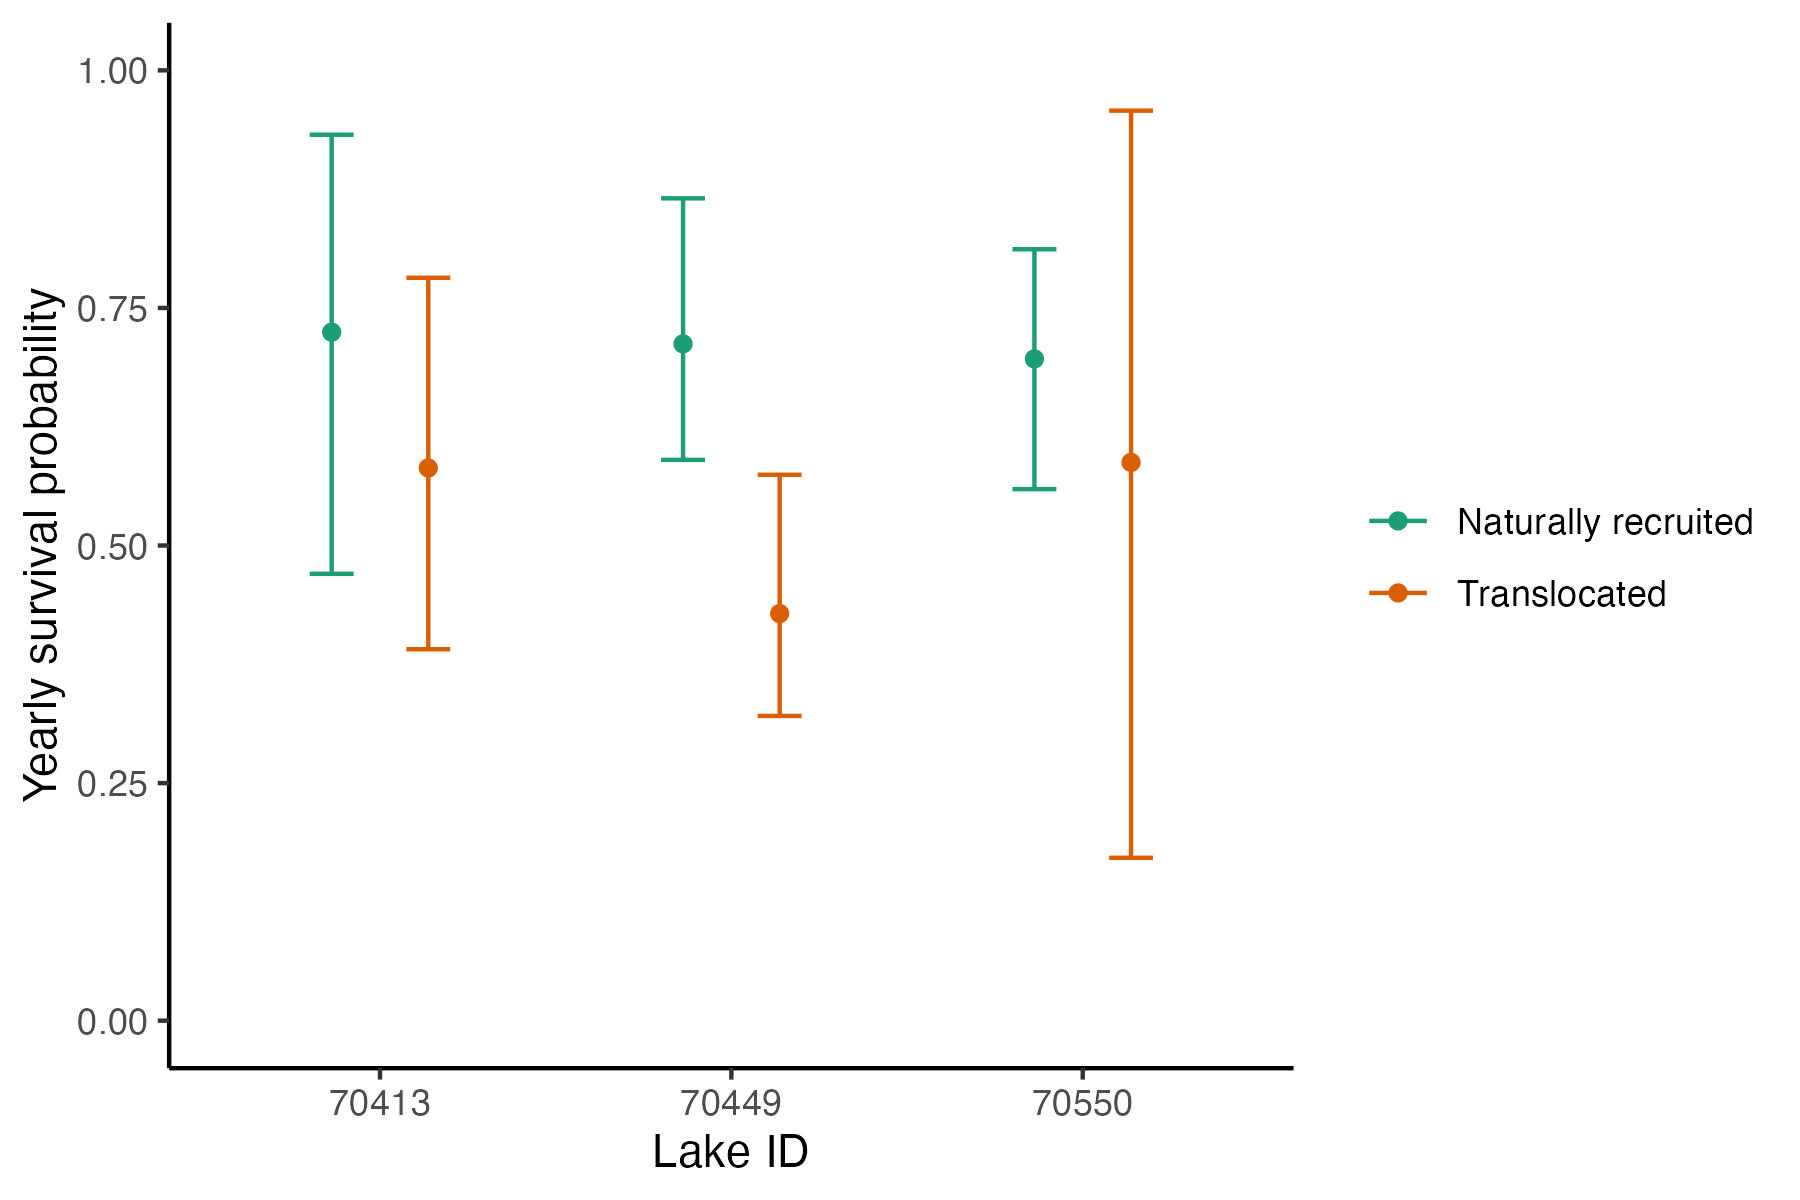
\includegraphics[width=6.04167in,height=\textheight]{figures/compare_surv_probs.jpg}

}

\caption{\label{fig-compare_surv_probs}Comparison of average yearly
adult survival probabilities for adults translocated to each of 3 sites
versus adults that were naturally recruited at each site (as a result of
reproduction by translocated frogs). In contrast to
Figure~\ref{fig-translocation-survival}, these are not survival
probabilities from the first year following translocation, but instead
represent averaged survival probabilities across multiple years and
cohorts. Points are median estimates and error bars give the 95\%
uncertainty intervals around the estimates, accounting for yearly
variation in survival probabilities. All estimates were derived using
the mrmr package, and the methods for calculation are described in
\textbf{Supporting Information - Population viability modeling -
Estimating model parameters}.}

\end{figure}

\newpage

\begin{figure}

{\centering 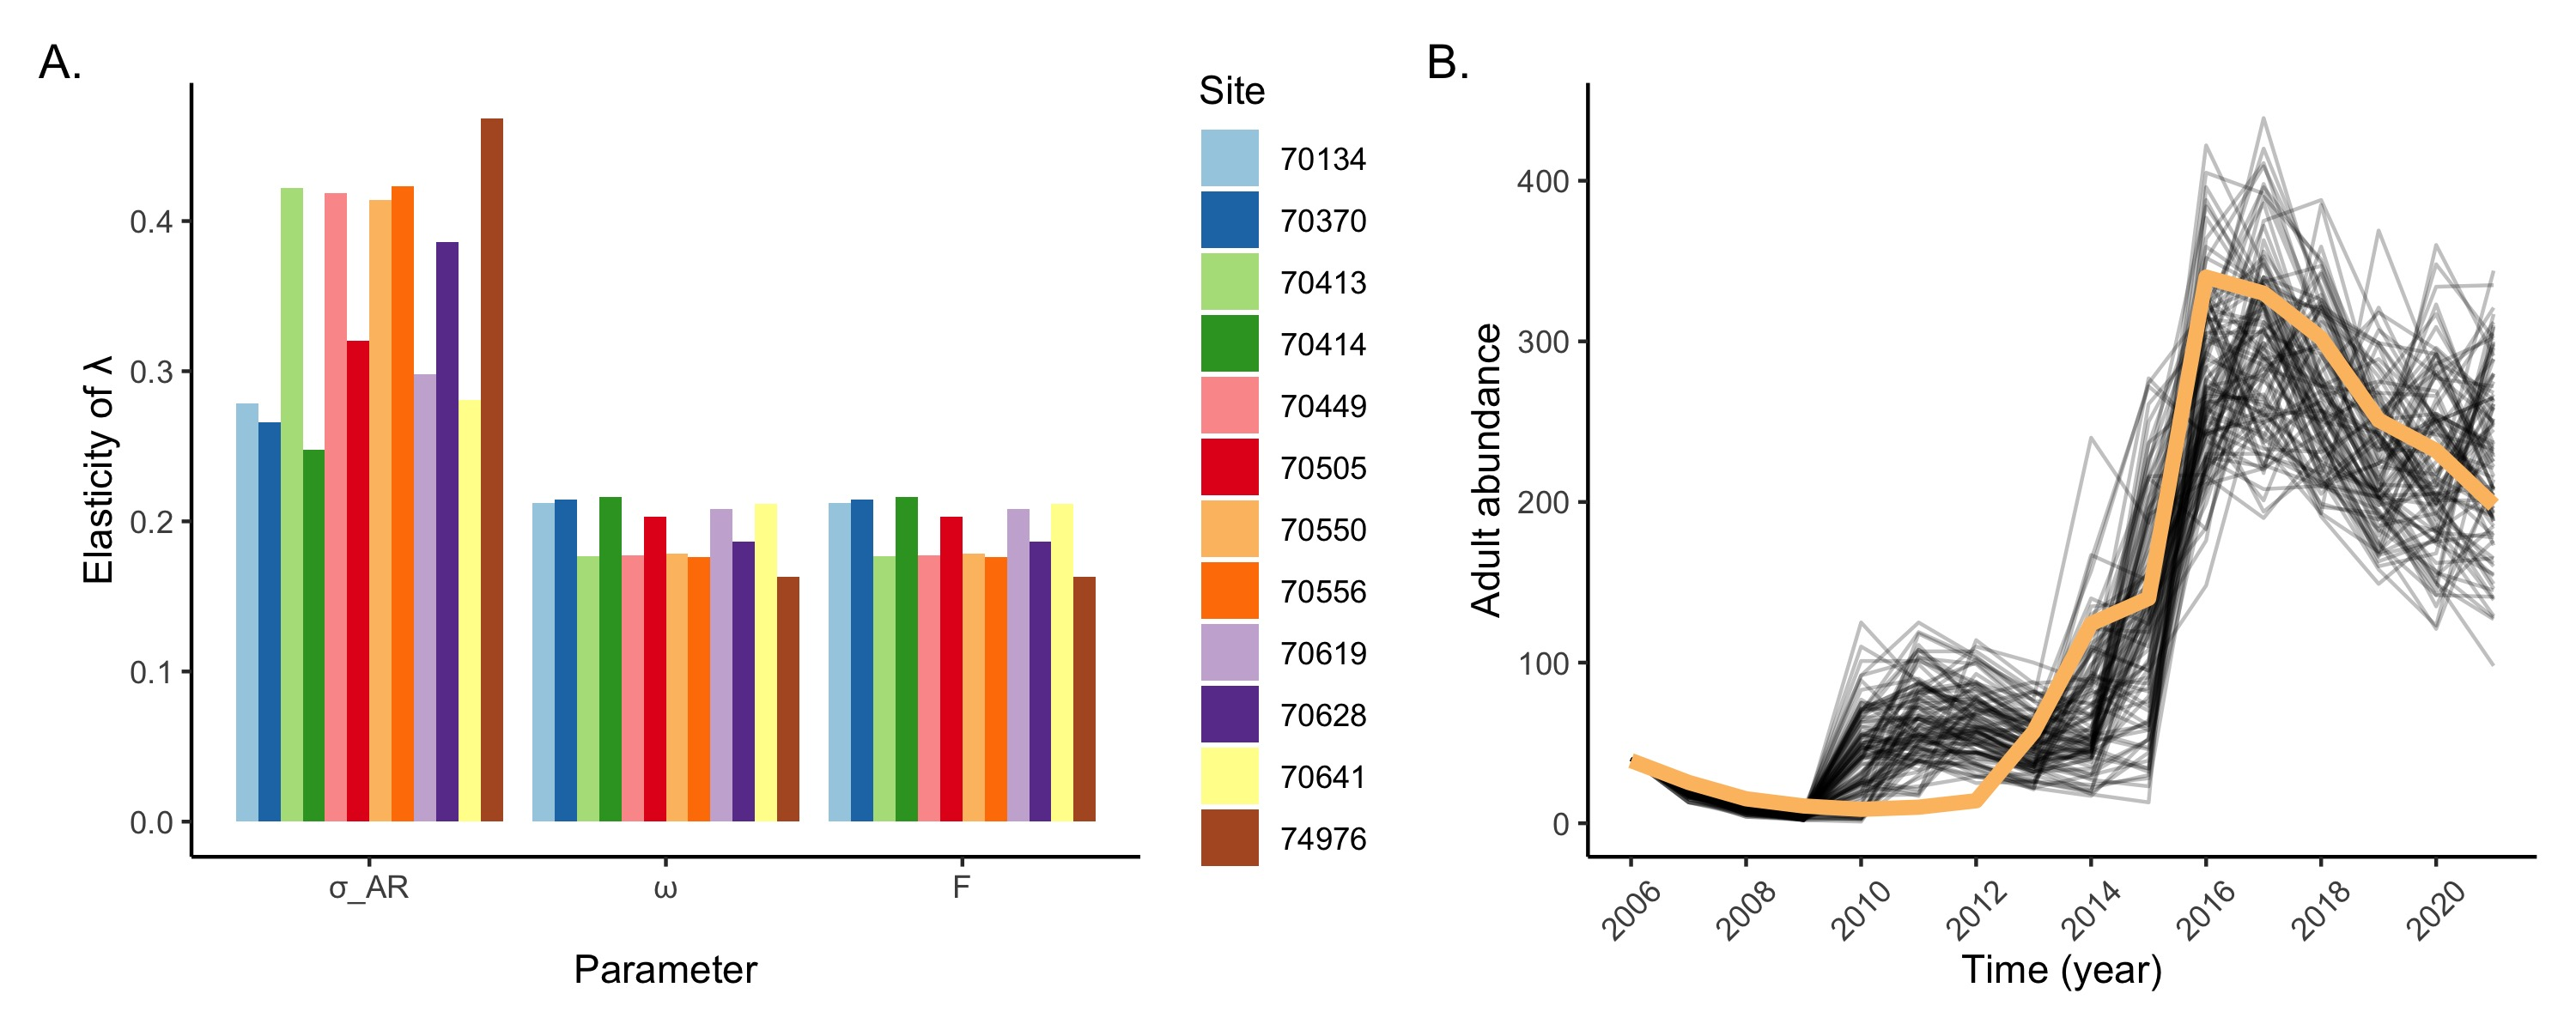
\includegraphics[width=5.72917in,height=\textheight]{figures/pop_viability_figures_for_supp.jpg}

}

\caption{\label{fig-viability-supp}Sensitivity analysis of the
stage-structured MYL frog model. Elasticity of \(\lambda\) with changes
in four parameters: \(\sigma_{A_R}\) (yearly survival probability of
naturally recruited adults), \emph{F (}number of eggs produced by a
female frog in a year that successfully hatch), \(\sigma_{J_1}\) (yearly
probability of survival of year-1 juveniles that also affects
recruitment), and \(\sigma_{J_2}\) (yearly probability of survival and
recruitment of year-2 juveniles). Elasticity is calculated at the
default parameter values for each population and \(\sigma_{J_1}\) =
0.09.}

\end{figure}

\newpage

\begin{figure}

{\centering 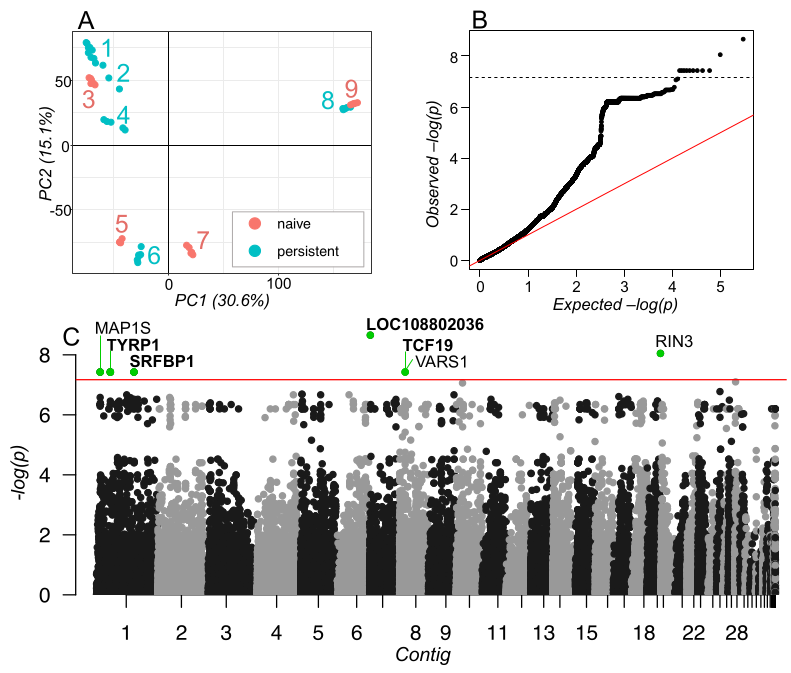
\includegraphics[width=5.72917in,height=\textheight]{figures/pca_qq_manhattan.png}

}

\caption{\label{fig-selectionresults}Results from the analysis of
individual variants, showing putative signatures of selection in
recovering MYL frog populations. (A) PCA calculated from binary SNPs
showing the genomic relationship of samples. Numeric labels and colors
match those in Figure~\ref{fig-allelefrequencies}. Populations 1-7 are
\emph{R. sierrae} and populations 8 and 9 are \emph{R. muscosa}. (B)
qqplot showing observed and expected p-values for 148,307 SNPs and
INDELS. Dashed line shows p-value that identifies outliers. (C)
Manhattan plot showing p-value for each SNP. SNPs are sorted by genomic
position and contigs are sorted by size. Red line shows p-value that
identifies outliers. Outlier SNPs above this threshold are highlighted
and labeled. Bold labels indicate the presence of at least one
non-synonymous SNP in that gene.}

\end{figure}

\newpage

\begin{figure}

{\centering 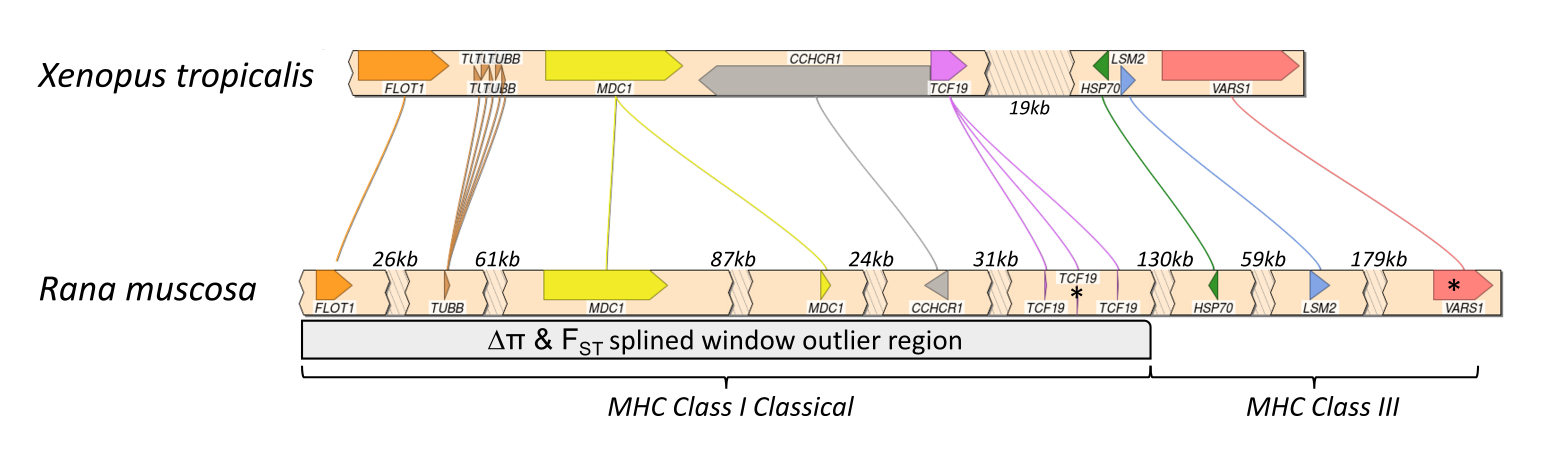
\includegraphics[width=6.77083in,height=\textheight]{figures/synteny_figure.png}

}

\caption{\label{fig-synteny-plot}Synteny plot showing conserved gene
order in \emph{Xenopus tropicalis} and \emph{Rana muscosa} for the
outlier region containing MHC Class I Classical and MHC Class III gene
regions. The plot was created with SimpleSynteny \citep{veltri2016}
using \emph{Xenopus tropicalis} Chromosome 8 (NC\_030684.2, genbank
accession GCA\_000004195.4) and \emph{Rana muscosa} Contig19. Asterices
indicate the location of SNP outliers in the TCF19 and VARS1 genes. Gap
sizes for each contig representation are labeled.}

\end{figure}

\newpage

\begin{figure}

{\centering 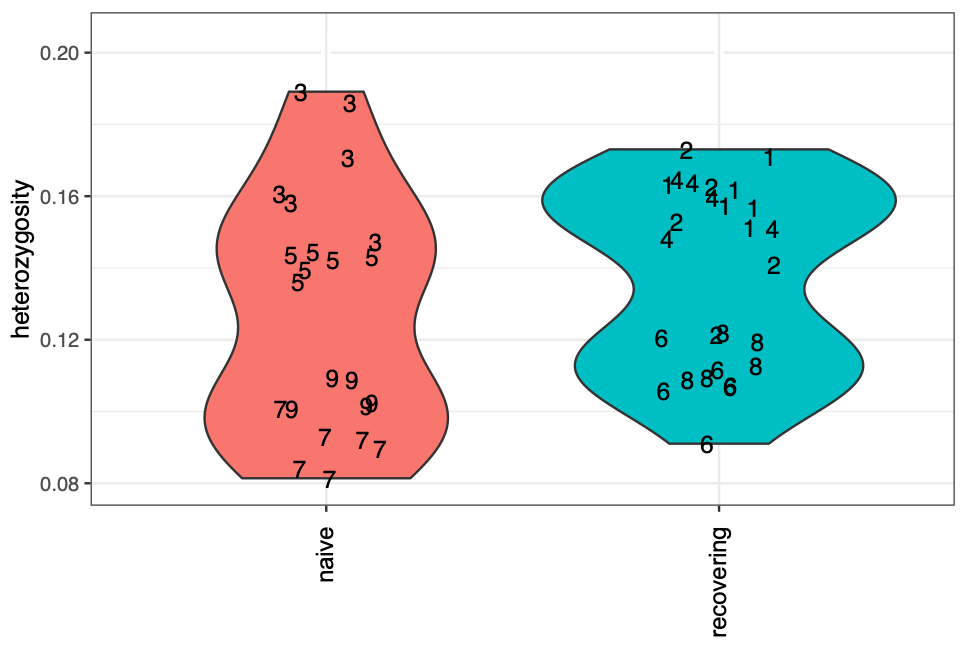
\includegraphics[width=5.20833in,height=\textheight]{figures/violin_plot_heterozy_by_group.png}

}

\caption{\label{fig-violinplot-heterozy}Violin plots showing individual
heterozygosity for the Bd-naive and recovering populations included in
the frog evolution study. Individual data points are represented by
their corresponding site number (from
Figure~\ref{fig-allelefrequencies}).}

\end{figure}

\newpage

\begin{figure}

{\centering 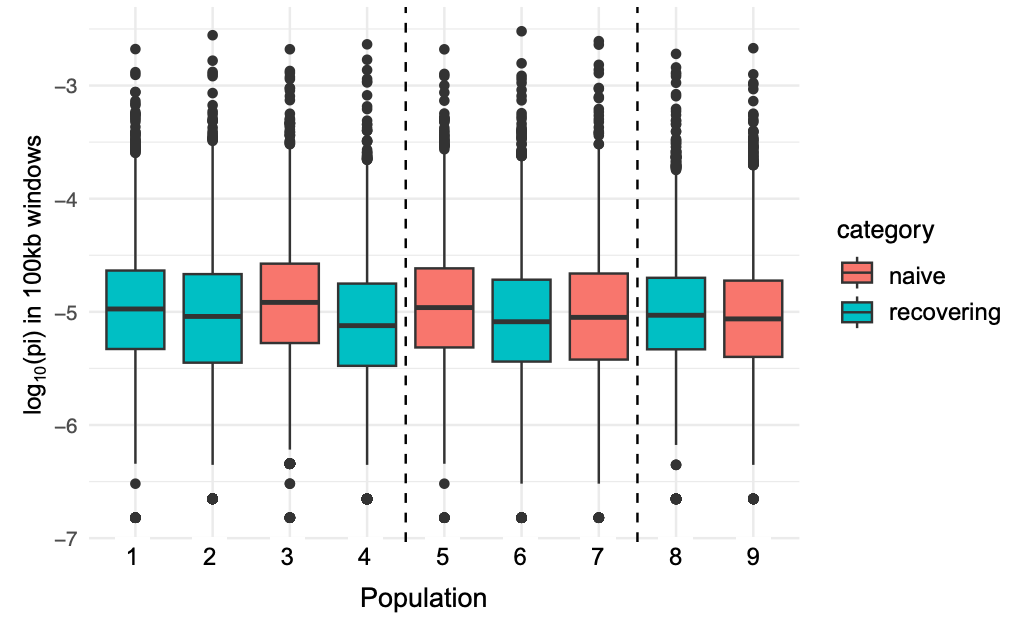
\includegraphics[width=5.72917in,height=\textheight]{figures/boxplot_genomewide_pi_by_pop.png}

}

\caption{\label{fig-boxplot-genomewide-pi-by-pop}For each study
population in the frog evolution study (from
Figure~\ref{fig-allelefrequencies}), boxplots showing nucleotide
diversity (\(\pi\)) within 100kb sliding windows along the genome. The
y-axis has been log\textsubscript{10}-transformed for display purposes.
Sites are color-coded as ``Bd-naive'' or ``recovering'', and vertical
dashed lines show the genetic breaks between frog populations as
described in Figure~\ref{fig-selectionresults} A SI).}

\end{figure}

\newpage

\begin{figure}

{\centering 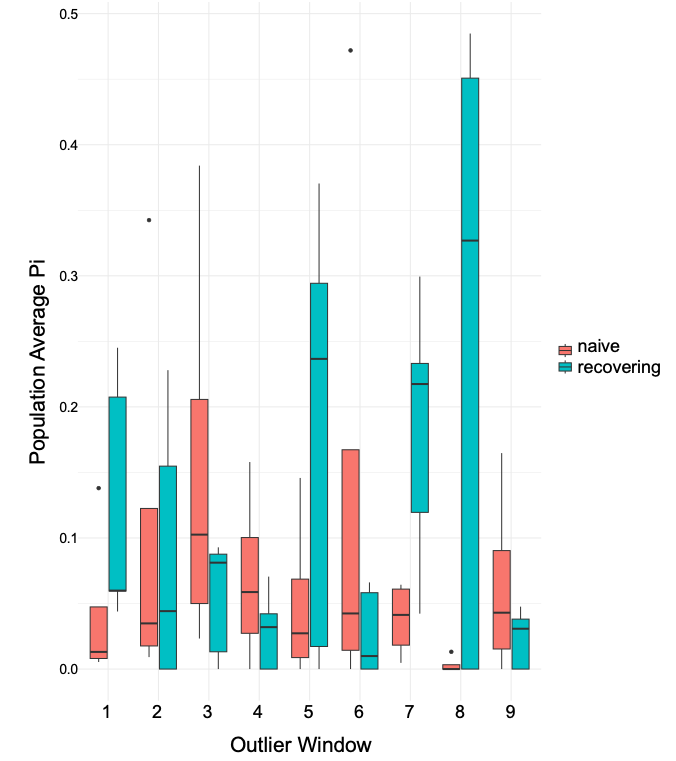
\includegraphics[width=5.20833in,height=\textheight]{figures/boxplot_pi_by_windowpop.png}

}

\caption{\label{fig-boxplot-pi-by-windowpop}For each of the 9 outlier
windows identified by the overlapping splined windows for FST and
\(\pi\), boxplots showing average \(\pi\) for naive and recovering
populations. The corresponding gene annotations for each window are as
follows: (1) C6, C7, (2) DDX10, ZBTB24, (3) SULTR-like, TRAF3IP2, VGLL3,
EXOC1, (4) FLOT1, TUBB, MDC1, CCHCR1, TCF19, HSP70, LSM2, VARS1, (5)
GCC2, CFAP251, PEG10, (6) ERO1A, GVINP1, (7) PPP1R12A, TSPAN4, PAWR,
MFRP, MAX, PPP6R3, (8) C6H5ORF22, PKS6, BSPRY, MPV17, and (9) CAD,
ATRAID, GPN1.}

\end{figure}

\newpage

\hypertarget{tables}{%
\subsubsection{Tables}\label{tables}}

\hypertarget{tbl-param_values}{}
\begin{longtable}[]{@{}
  >{\raggedright\arraybackslash}p{(\columnwidth - 4\tabcolsep) * \real{0.3611}}
  >{\raggedright\arraybackslash}p{(\columnwidth - 4\tabcolsep) * \real{0.2639}}
  >{\raggedright\arraybackslash}p{(\columnwidth - 4\tabcolsep) * \real{0.3750}}@{}}
\caption{\label{tbl-param_values}Description and values of parameters
used in the model. All survival probabilities are in the presence of the
fungal pathogen Bd.}\tabularnewline
\toprule()
\begin{minipage}[b]{\linewidth}\raggedright
\textbf{Parameter}
\end{minipage} & \begin{minipage}[b]{\linewidth}\raggedright
\textbf{Value}
\end{minipage} & \begin{minipage}[b]{\linewidth}\raggedright
\textbf{Source}
\end{minipage} \\
\midrule()
\endfirsthead
\toprule()
\begin{minipage}[b]{\linewidth}\raggedright
\textbf{Parameter}
\end{minipage} & \begin{minipage}[b]{\linewidth}\raggedright
\textbf{Value}
\end{minipage} & \begin{minipage}[b]{\linewidth}\raggedright
\textbf{Source}
\end{minipage} \\
\midrule()
\endhead
\(\sigma_{L_1}\), Yearly survival probability of year-1 tadpoles & 0.7 &
Estimated from field data, observations, natural history knowledge \\
\(\sigma_{L_2}\), Yearly survival probability of year-2 tadpoles & 0.7 &
Estimated from field data, observations, natural history knowledge \\
\(\sigma_{L_3}\), Yearly survival probability of year-3 tadpoles & 0.7 &
Estimated from field data, observations, natural history knowledge \\
\(\sigma_{J_1}\), Yearly survival probability of year-1 juveniles &
Varies yearly & Varies. Bounds estimated from field data, observations,
natural history knowledge \\
\(\sigma_{J_2}\), Yearly survival probability of year-2 juveniles & 0.5
& Estimated from field data, observations, natural history knowledge \\
\(\sigma_{A_R}\), Yearly survival probability of naturally recruited
adults & Varies by population & Estimated from CMR studies \\
\(\sigma_{A_T}\), Yearly survival probability of translocated adults &
Varies by population & Estimated from CMR studies \\
\(p_{L_1}\), Probability of a year-1 tadpoles remaining as a tadpoles &
1 & Estimated from field data, observations, natural history
knowledge \\
\(p_{L_2}\), Probability of a year-2 tadpoles remaining as a tadpoles &
0.25 & Estimated from field data, observations, natural history
knowledge \\
\(p_{J_1}\), Probability of a year-1 juvenile remaining as a juvenile &
0.25 & Estimated from field data, observations, natural history
knowledge \\
\(p_F\), Probability of a adult female reproducing in a year & 0.5 &
Could be as high at 1, based on field observations \\
\(F\), Number of surviving eggs produced by an adult female & 100 & From
observations of captive frogs \\
\bottomrule()
\end{longtable}

\newpage

\hypertarget{datasets}{%
\subsubsection{Datasets}\label{datasets}}

Dataset S1. Set of liberal SNP and INDEL outlier variants (Bonferroni
corrected p-value \textless{} 0.05), identified via GEMMA. file:
gemma\_outliers\_all.csv

Dataset S2. Set of strict SNP and INDEL outlier variants (Bonferroni
corrected p-value \textless{} 0.01), identified via GEMMA. Additional
information includes variant location within the gene
(predicted\_gene\_loc) and whether the variant is synonymous or
nonsynonymous (predicted\_effect\_AA). file:
gemma\_outliers\_strict\_freq.csv

Dataset S3. Description of overlapping \emph{F\textsubscript{ST}} and
\(\pi_{diff}\) outlier windows, as identified in the splined window
analysis. The outlier window on chromosome 19 (column name =
chr\_num\_sorted) is included twice because one
\emph{F\textsubscript{ST}} outlier window overlapped with two
\(\pi_{diff}\) outlier windows. file:
spline\_window\_shared\_outliers.csv

Dataset S4. Annotation information for all genes within each of the
overlapping outlier windows in dataset S3. file:
spline\_window\_gene\_details

\hypertarget{references-1}{%
\subsubsection{References}\label{references-1}}


  \bibliography{translocation.bib}


\end{document}
